% =====================================================================
%  House LaTeX template: minimal, light (Piero). Shared by report/ and results/.
% =====================================================================
\documentclass[11pt]{article}

% ---------- PAGE ----------
\usepackage[a4paper,margin=2.1cm,headheight=14pt,footskip=26pt]{geometry}
\setlength{\parindent}{0pt}
\setlength{\parskip}{0.55em}
\IfFileExists{lmodern.sty}{\usepackage[T1]{fontenc}\usepackage{lmodern}}{}
\usepackage{microtype}
\usepackage{amsmath,amssymb}
\linespread{1.04}

% ---------- COLOURS (Berkeley) ----------
\usepackage[dvipsnames]{xcolor}
\definecolor{bblue}{HTML}{003262}   % Berkeley Blue
\definecolor{bgold}{HTML}{FDB515}   % California Gold
\definecolor{ink}{HTML}{16181D}
\definecolor{mute}{HTML}{6B7280}
\definecolor{hair}{HTML}{D4D8DE}
\definecolor{paper}{HTML}{F5F6F8}
\definecolor{confc}{HTML}{003262}   % confirmatory
\definecolor{posthc}{HTML}{B35C00}  % post-hoc
\definecolor{fwdc}{HTML}{2E7D32}    % forward test
\color{ink}

% ---------- PACKAGES ----------
\usepackage{graphicx}
\usepackage{booktabs,tabularx,array,threeparttable,multirow}
\newcolumntype{Y}{>{\raggedright\arraybackslash}X}
\setlength{\aboverulesep}{0.3ex}\setlength{\belowrulesep}{0.5ex}
\usepackage{float}
\usepackage[font=small,labelfont={color=bblue,sc},labelsep=period,skip=5pt,justification=raggedright,singlelinecheck=false]{caption}
\usepackage{subcaption}
\usepackage[shortlabels]{enumitem}
\setlist{itemsep=1pt,topsep=2pt,parsep=0pt}
\usepackage{titlesec}
\usepackage{fancyhdr}
\usepackage[most]{tcolorbox}
\usepackage{listings}
\usepackage{tikz}
\usetikzlibrary{arrows.meta,positioning,calc}
\usepackage[round,authoryear]{natbib}
\usepackage[colorlinks=true,linkcolor=bblue,citecolor=bblue,urlcolor=bblue]{hyperref}
\usepackage[capitalise,noabbrev]{cleveref}

% ---------- REPORT INFO ----------
\newcommand{\ReportTitle}{Follow the Workers}
\newcommand{\ReportSubtitle}{Do labor-market flows predict which U.S.\ industries outperform?}
\newcommand{\CourseName}{MFE 230GA \textendash{} Equity Markets}
\newcommand{\CourseShort}{MFE 230GA}
\newcommand{\Term}{Fall 2026}
\newcommand{\SubmitDate}{October 4, 2026}

% ---------- SECTIONS (bold only in titles) ----------
\titleformat{\section}{\large\bfseries\color{bblue}}{\thesection}{0.7em}{}[{\color{hair}\titlerule[0.5pt]}]
\titlespacing*{\section}{0pt}{16pt}{8pt}
\titleformat{\subsection}{\normalsize\bfseries}{\textcolor{bblue}{\thesubsection}}{0.7em}{}
\titlespacing*{\subsection}{0pt}{11pt}{3pt}
\titleformat{\paragraph}[runin]{\normalsize\itshape}{}{}{}[.]
\titlespacing*{\paragraph}{0pt}{6pt}{0.6em}

% ---------- HEADER / FOOTER ----------
\pagestyle{fancy}\fancyhf{}
\renewcommand{\headrulewidth}{0pt}
\renewcommand{\footrulewidth}{0.4pt}
\renewcommand{\footrule}{{\color{hair}\hrule width\headwidth height\footrulewidth\vskip\footruleskip}}
\fancyhead[R]{\footnotesize\color{mute}Page \thepage}
\fancyfoot[L]{\footnotesize\color{mute}\CourseShort{} \textperiodcentered{} Final Project}
\fancyfoot[R]{\footnotesize\color{mute}\ReportTitle}

% ---------- LABELS, DRAFT MARKS ----------
\newif\ifdraft \drafttrue   % \draftfalse for the submission build
\DeclareRobustCommand{\pill}[2]{\tcbox[on line,colback=#1!9,colframe=#1!9,boxrule=0pt,arc=1.6pt,
  left=2.5pt,right=2.5pt,top=0.5pt,bottom=0.5pt,boxsep=0pt]{\textcolor{#1}{\scriptsize\textsc{#2}}}}
\DeclareRobustCommand{\tagc}{\pill{confc}{confirmatory}}
\DeclareRobustCommand{\tagp}{\pill{posthc}{post-hoc}}
\DeclareRobustCommand{\tagf}{\pill{fwdc}{forward test}}
\newcommand{\prov}[1]{\ifdraft{\setlength{\fboxsep}{1pt}\colorbox{bgold!30}{#1}}\else #1\fi}
\newcommand{\todo}[1]{\ifdraft{\color{red!70!black}\footnotesize[TODO: #1]}\fi}

% ---------- BOXES ----------
\newtcolorbox{keybox}[1][]{enhanced,breakable,sharp corners,frame hidden,boxrule=0pt,
  colback=paper,borderline west={2pt}{0pt}{bgold},left=9pt,right=9pt,top=5pt,bottom=6pt,
  fontupper=\small,before upper={\ifx\relax#1\relax\else{\textcolor{bblue}{\textsc{#1}}\par\smallskip}\fi}}
\newtcolorbox{promptbox}[1]{enhanced,breakable,sharp corners,frame hidden,boxrule=0pt,
  colback=paper,borderline west={2pt}{0pt}{bblue},left=9pt,right=9pt,top=5pt,bottom=6pt,
  before upper={{\small\textcolor{bblue}{\textsc{#1}}}\par\smallskip\raggedright\footnotesize\ttfamily}}

% ---------- CODE ----------
\lstset{language=Python,basicstyle=\ttfamily\footnotesize,columns=fullflexible,keepspaces,
  breaklines,showstringspaces=false,frame=leftline,framerule=2pt,rulecolor=\color{bblue},
  backgroundcolor=\color{paper},xleftmargin=8pt,framexleftmargin=8pt,aboveskip=6pt,belowskip=6pt,
  keywordstyle=\color{bblue},commentstyle=\color{mute}\itshape,stringstyle=\color{posthc}}

% ---------- COVER ----------
\newcommand{\BerkeleyMark}{%
  \IfFileExists{figures/berkeley_mfe_logo.pdf}{\includegraphics[height=1.4cm]{figures/berkeley_mfe_logo.pdf}}{%
  \IfFileExists{figures/berkeley_mfe_logo.png}{\includegraphics[height=1.4cm]{figures/berkeley_mfe_logo.png}}{%
  {\color{bblue}\fontsize{24}{26}\selectfont\bfseries Berkeley}\hspace{0.7em}%
  {\color{bgold}\rule[-3pt]{1.4pt}{22pt}}\hspace{0.7em}%
  \parbox[b]{7cm}{\color{bblue}\footnotesize\textsc{Haas School of Business}\\[-1pt]\textsc{Master of Financial Engineering}}}}}

\newcommand{\MakeCover}{%
\begin{titlepage}
\newgeometry{margin=2.5cm}
\BerkeleyMark
\vspace*{0.26\textheight}

{\raggedright
{\color{mute}\small\textsc{\CourseShort{} \textperiodcentered{} Final Project \textperiodcentered{} \Term}}\par\vspace{10pt}
{\fontsize{34}{38}\selectfont\bfseries\color{bblue}\ReportTitle\par}
\vspace{10pt}
{\Large\color{mute}\ReportSubtitle\par}
\vspace{18pt}
{\color{bgold}\rule{3.2cm}{1.6pt}}\par}

\vfill
\begin{minipage}[t]{0.46\textwidth}
{\color{mute}\footnotesize\textsc{Team}}\par\vspace{4pt}
\begin{tabular}{@{}l l@{}}
Piero    & \textsc{Pelosi} \\
Alex     & \textsc{Roesler} \\
Romain   & \textsc{Almeida} \\
Elouan   & \textsc{Bahri} \\
Al Yazid & \textsc{Bensaid}
\end{tabular}
\end{minipage}\hfill
\begin{minipage}[t]{0.46\textwidth}
{\color{mute}\footnotesize\textsc{Course}}\par\vspace{4pt}
\CourseName\par\vspace{8pt}
{\color{mute}\footnotesize\textsc{Instructors}}\par\vspace{4pt}
Raffaele Savi and Gerald Garvey\par{\small\color{mute}BlackRock}\par\vspace{8pt}
{\color{mute}\footnotesize\textsc{Graduate Student Instructor}}\par\vspace{4pt}
Vinicio DeSola
\end{minipage}

\vspace{1.4cm}
{\color{hair}\rule{\textwidth}{0.5pt}}\par\vspace{2pt}
{\footnotesize\color{mute}UC Berkeley Haas \textperiodcentered{} Master of Financial Engineering\hfill\SubmitDate}
\restoregeometry
\end{titlepage}
\setcounter{page}{1}}

\renewcommand{\ReportTitle}{Follow the Workers: Results Book}
\renewcommand{\ReportSubtitle}{Every result, figure, table and claim behind the report, with its source file}
\usepackage{longtable}
\begin{document}
\MakeCover
\tableofcontents
\clearpage
\section{Verdict}
\IfFileExists{verdict.tex}{% Verdict page of the Results Book; prose mirrors results/VERDICT.md. Claim IDs refer to results/claims.csv.
\subsection*{Verdict on each strategy}
{\small\setlength{\tabcolsep}{4pt}
\begin{tabularx}{\textwidth}{@{}p{3.4cm} l Y@{}}
\toprule
Strategy & Label & Verdict \\
\midrule
A3, preregistered primary & \tagc & \emph{Do not implement.} Test Sharpe $-0.58$, IC $-0.021$ ($t=-1.08$), placebo $p=0.72$, fails gates G2--G5. Nothing below changes this. [C01--C07] \\
A0, A1, A1-T, A4 & \tagc & Negative in the test ($-0.36$ to $-0.79$); not primary; no claim. [C08] \\
Opus follow-up, A4 & expl. & Launched after the test was seen. Sharpe $+0.01$ but IC $t=-0.10$, alpha $t=0.05$, fails G2--G5; its gross came from one long industry. Evidence about agents, not the strategy. [X01, X02, X04] \\
V2a wage growth (declared headline) & \tagp & Modest and fragile: test Sharpe $+0.16$, IC $+0.049$ ($t=2.04$), placebo $p=0.02$, but alpha $t=0.29$, a value/momentum tilt (HML $-0.43$, Mom $+0.22$), Sharpe $-1.71$ in the last 18 months, DSR 0.02. Not distinguishable from noise after the looks taken. Forward-tested. [V\_V2a\_SR, V01, V11] \\
V2b signed composite & \tagp & Negative (test $-0.15$); learned signs did not help. [V\_V2b\_SR, V06] \\
V2c wage + momentum & \tagp & Test $+0.35$, alpha $t=1.36$, placebo $p=0.26$, DSR 0.09; momentum supplies the return. Its ETF book has four legs. [V\_V2c\_SR, V05, F04] \\
V2d $-$(hires + quits), 12-month hold & \tagp & \emph{The thesis result, fragile in time.} Positive in every window ($+0.50$ research, $+0.29$ test, $+0.35$ full, $+0.29$ last 18m); 12-month IC $+0.096$ ($t=2.43$) against a 1-month IC of $-0.02$; alpha $+0.26\%$ a month ($t$ 1.5 test, 1.9 full); survives components, holding 9--18 months, 50\,bp costs (break-even 68\,bp) and every drop-one run (min $+0.18$). Fails one pre-declared condition: first test half $-0.21$ (second $+0.64$); the test bootstrap interval includes zero; DSR 0.05 at 132 trials. Not tradeable on this evidence; the forward test is live. [V\_V2d\_SR, V02, V03, R1a--R9a, R12, R13] \\
\bottomrule
\end{tabularx}}

\subsection*{The story in one paragraph}
Public labor flows do carry information about industry returns, but as slow cost news rather than fast demand news. The preregistered strategy traded the fast channel: it bet that industries with rising openings, hires and hours would outperform next month, and it lost money in a one-time test on 142 untouched months (Sharpe $-0.58$). Two of its four signs were wrong and the one stable short-horizon signal, wage growth, had been dropped during the build. When we look at horizons instead of months, the picture inverts: industries that hire and lose workers fastest earn lower returns over the following 9 to 24 months, as investment-based asset pricing predicts, and a 12-month book built on that sign (V2d) is positive in every window we have. That book was designed after the test was opened, it was negative in the first half of the test, and its deflated Sharpe is near zero, so it is a hypothesis with a live forward test, not an implementable strategy. The verdict is still \emph{Do not implement}.

\subsection*{What we can claim}
\begin{itemize}
\item The preregistered strategy fails cleanly and we know why: wrong signs [D03], wrong horizon [D04, R2a], an untestable moderator [D06, D07], agent features active in 3 test months [D12], over-shrinkage and a binding risk cap [C18, D13], concentrated losses [D09]. Costs were not the cause [C15].
\item Wage growth is the only short-horizon labor signal whose IC exceeds 1.5 standard errors in both periods [D01]; both blinded agent runs rediscovered it.
\item Hiring and quits predict returns with a negative sign at 9--24 months and not at 1 month [R2a, R2b]; hires alone carry most of it [R1a, R1b].
\item V2d is not carried by one industry [R7a], survives realistic costs [R5a] and longer holding periods [R3a], and FF5 + momentum do not explain it (alpha $t$ 1.5--1.9) [R6a, R6a2], but it loads against profitability [R6b].
\item The 13-group universe caps what any IC can deliver: a 0.1 twelve-month IC with breadth 13 implies an IR near 0.35 at best; V2a realised far less than its IC implied [R11a].
\item A stronger model followed the protocol better but found no more out-of-sample signal; the LLM judge over-attributed idea uptake [A01, A02, A03, D10].
\item The forward test is frozen and the Q4 2026 books are dollar-neutral [F01--F05].
\end{itemize}

\subsection*{What we cannot claim}
\begin{itemize}
\item That any post-hoc variant passed: none met the v2 reading rule [V07]; V2d fails R4 and its test bootstrap interval includes zero [R9a, R13]; every DSR is below 0.2 [V08, R12].
\item That V2d is tradeable, or that the tightness pattern in R8 is more than one draw with 54--88 months per cell [R8a].
\item Anything about as-known data for v2/v3: all historical v2/v3 numbers use revised data with fixed lags [R10, S02].
\item That the Opus study's $+0.01$ is evidence for the strategy [X01].
\item Alpha from the labor signal beyond quality/growth exposure for A3 or V2a [C13, V11].
\end{itemize}

\subsection*{Figure plan for the report}
1 \path{fig_timeline} [D06], 2 \path{fig_agents} [A01, A02], 3 \path{fig_loadings} [C13, V11, R6b], 4 \path{fig_cumulative} [C08, V2a], 5 \path{fig_ic_signals} [D01--D03], 6 \path{fig_horizon} [D04, D05], 7 \path{fig_agents_scatter} [D10--D12], 8 \path{fig_horizon_profile} [R2a, R2b], 9 \path{fig_v2_windows} [V2a--V2d Sharpe], 10 \path{fig_v2d_dropone} [R7a]; appendix: \path{fig_tightness}, \path{fig_v2d_tightness}, \path{fig_industry_pnl}, \path{fig_v2d_holding}.
}{\emph{VERDICT.md is written at Stage 3.}}
\section{Scoreboard}
The A3 sealed ledger starts from an empty book in November 2014; the v2 test figures are the test slice of a continuous run that starts in May 2004 (pre-declared in v2\_spec.md section 4). IC is one-month except HQ12 (12-month, its holding horizon). DSR is the research-period value with 41 nominal trials for the frozen studies and the test-window value with 112 trials for v2. Labels: conf.\ = confirmatory, expl.\ = exploratory follow-up. Source: \path{results/scoreboard.csv}.
{\scriptsize\setlength{\tabcolsep}{3pt}\begin{tabular}{@{}p{2.9cm} l r r r r r r r r p{2.3cm}@{}}
\toprule
Strategy & Label & Res. & Test & Full & 18m & IC ($t$) & $\alpha$/m ($t$) & Plac. & DSR & Verdict \\
\midrule
A0 fixed rule (Sonnet) & conf. & $-$0.44 & $-$0.36 & $-$0.48 & $-$1.56 & $-$0.020 ($-$0.71) & $-$0.25\% ($-$0.92) &  & 0.00 & negative, not primary \\
A1 ridge (Sonnet) & conf. & $-$0.54 & $-$0.51 & $-$0.52 & +0.73 & $-$0.014 ($-$0.74) & $-$0.35\% ($-$1.72) &  & 0.00 & negative, not primary \\
A1-T tightness (Sonnet) & conf. & $-$0.55 & $-$0.59 & $-$0.58 & $-$0.37 & $-$0.029 ($-$1.42) & $-$0.42\% ($-$2.06) &  & 0.00 & negative, not primary \\
A3 primary (Sonnet) & conf. & $-$0.13 & $-$0.58 & $-$0.44 & +0.85 & $-$0.021 ($-$1.08) & $-$0.38\% ($-$1.86) & 0.72 & 0.00 & Do not implement \\
A4 islands (Sonnet) & conf. & $-$0.18 & $-$0.79 & $-$0.56 & +1.23 & $-$0.020 ($-$0.86) & $-$0.55\% ($-$2.39) &  & 0.00 & negative, not primary \\
A3 (Opus follow-up) & expl. & $-$0.48 & $-$0.46 & $-$0.46 & $-$0.64 & +0.001 (+0.05) & $-$0.24\% ($-$1.54) &  & 0.00 & exploratory, negative \\
A4 primary (Opus follow-up) & expl. & $-$0.40 & +0.01 & $-$0.13 & $-$1.41 & $-$0.002 ($-$0.10) & +0.01\% (+0.05) & 0.56 & 0.00 & exploratory, fails G2--G5 \\
V2a wage growth (headline) & post-hoc & +0.09 & +0.16 & +0.15 & $-$1.71 & +0.049 (+2.04) & +0.06\% (+0.29) & 0.02 & 0.02 & noise after the looks taken \\
V2b signed composite & post-hoc & $-$0.06 & $-$0.15 & $-$0.11 & $-$1.34 & +0.042 (+1.65) & $-$0.18\% ($-$0.84) & 0.05 & 0.00 & noise after the looks taken \\
V2c wage + momentum & post-hoc & +0.27 & +0.35 & +0.32 & $-$0.78 & +0.032 (+1.21) & +0.22\% (+1.36) & 0.26 & 0.09 & noise after the looks taken \\
V2d -(hires+quits), 12m & post-hoc & +0.50 & +0.29 & +0.35 & +0.29 & +0.096 (+2.43) & +0.26\% (+1.37) & 0.85 & 0.06 & noise after the looks taken \\
\bottomrule
\end{tabular}
}
\section{Figures}
\begin{figure}[H]\centering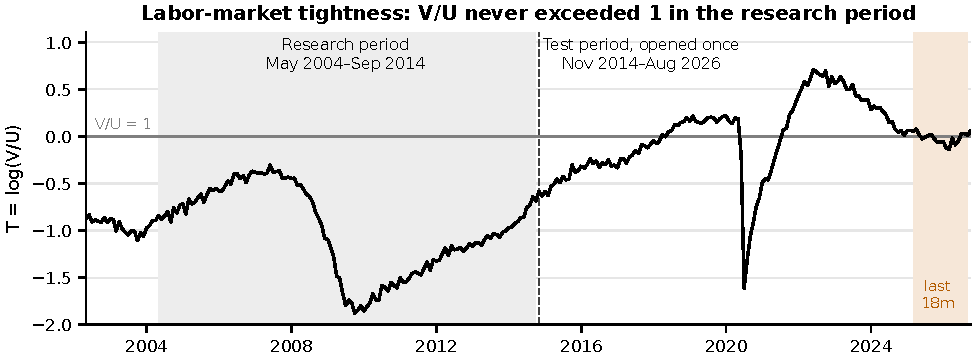
\includegraphics[width=\linewidth]{../report/figures/fig_timeline.pdf}\caption{Tightness never exceeded V/\allowbreak{}U = 1 in the research period, so the tightness moderator could not be learned there. \textcolor{mute}{\footnotesize Source: analysis/\allowbreak{}data/\allowbreak{}fred (JTSJOL, UNEMPLOY).} \hfill \tagp}\end{figure}
\begin{figure}[H]\centering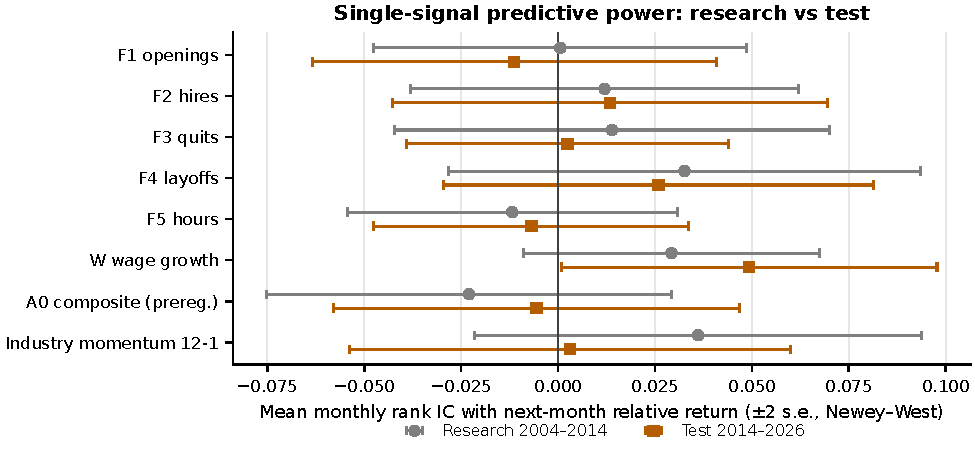
\includegraphics[width=\linewidth]{../report/figures/fig_ic_signals.pdf}\caption{Only wage growth has an IC above 1.5 standard errors in both periods; layoffs and hours carry the opposite sign to the one A0 imposed. \textcolor{mute}{\footnotesize Source: analysis/\allowbreak{}output/\allowbreak{}study1/\allowbreak{}tables/\allowbreak{}d1\_\allowbreak{}signal\_\allowbreak{}ic.csv.} \hfill \tagp}\end{figure}
\begin{figure}[H]\centering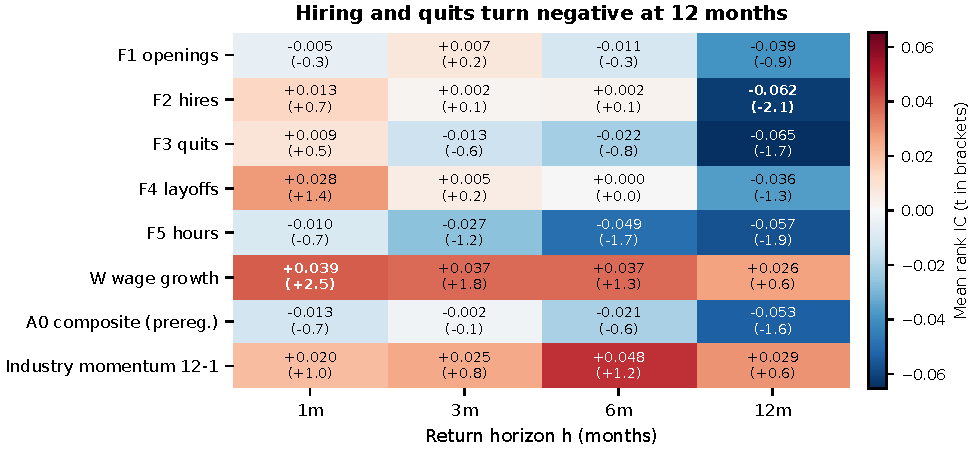
\includegraphics[width=\linewidth]{../report/figures/fig_horizon.pdf}\caption{Hires and quits turn negative at 12 months (t -2.1, -1.7): the investment/\allowbreak{}cost channel shows up slowly, not at one month. \textcolor{mute}{\footnotesize Source: analysis/\allowbreak{}output/\allowbreak{}study1/\allowbreak{}tables/\allowbreak{}d2\_\allowbreak{}horizon\_\allowbreak{}ic.csv.} \hfill \tagp}\end{figure}
\begin{figure}[H]\centering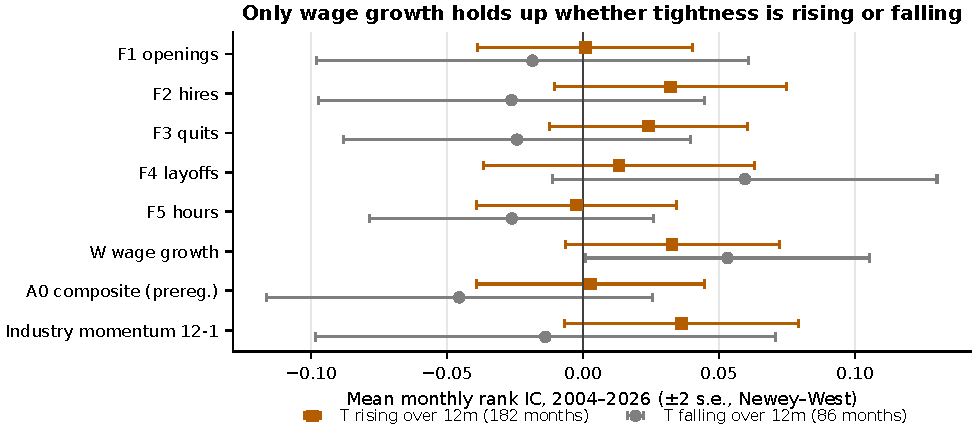
\includegraphics[width=\linewidth]{../report/figures/fig_tightness.pdf}\caption{Split by whether T rose or fell over 12 months, hires and quits predict returns only while the market tightens; the split is balanced in both periods. \textcolor{mute}{\footnotesize Source: analysis/\allowbreak{}output/\allowbreak{}study1/\allowbreak{}tables/\allowbreak{}d3\_\allowbreak{}tightness\_\allowbreak{}ic.csv.} \hfill \tagp}\end{figure}
\begin{figure}[H]\centering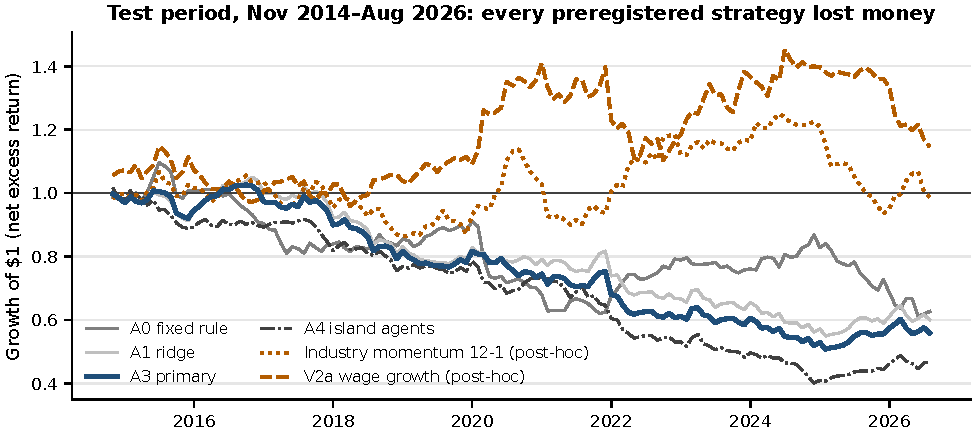
\includegraphics[width=\linewidth]{../report/figures/fig_cumulative.pdf}\caption{Every preregistered strategy lost money in the test; the post-hoc wage-growth book gained until 2024 and gave much of it back. \textcolor{mute}{\footnotesize Source: sealed/\allowbreak{}initial/\allowbreak{}ASOF\_\allowbreak{}*\_\allowbreak{}ledger.csv; analysis/\allowbreak{}output/\allowbreak{}study2/\allowbreak{}tables/\allowbreak{}v2\_\allowbreak{}monthly\_\allowbreak{}net.csv.} \hfill \tagc (A0-A4) / \tagp (momentum, W)}\end{figure}
\begin{figure}[H]\centering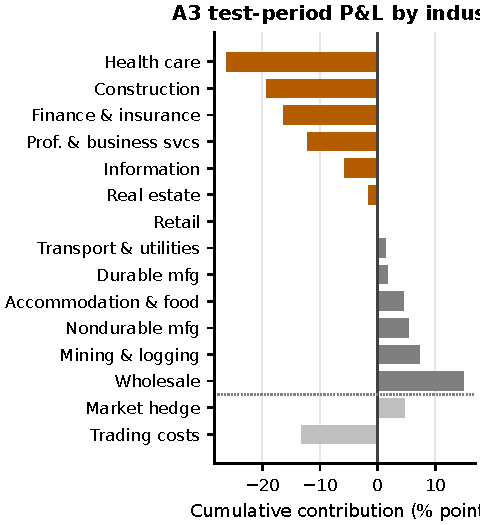
\includegraphics[width=\linewidth]{../report/figures/fig_industry_pnl.pdf}\caption{A3 lost most in health care, construction and finance; trading costs were a secondary drag. \textcolor{mute}{\footnotesize Source: analysis/\allowbreak{}output/\allowbreak{}study1/\allowbreak{}tables/\allowbreak{}d5\_\allowbreak{}industry\_\allowbreak{}pnl.csv.} \hfill \tagp}\end{figure}
\begin{figure}[H]\centering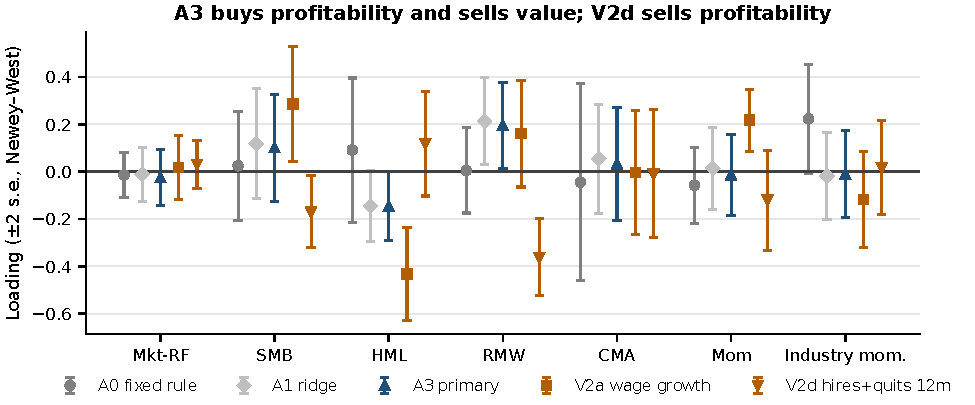
\includegraphics[width=\linewidth]{../report/figures/fig_loadings.pdf}\caption{The labor books are quality/\allowbreak{}growth tilts: A3 loads on RMW and against HML; W loads against HML and on momentum. \textcolor{mute}{\footnotesize Source: results.json attribution; analysis/\allowbreak{}output/\allowbreak{}study2/\allowbreak{}tables/\allowbreak{}v2a\_\allowbreak{}factor\_\allowbreak{}loadings\_\allowbreak{}test.csv.} \hfill \tagc (A0, A1, A3) / \tagp (W)}\end{figure}
\begin{figure}[H]\centering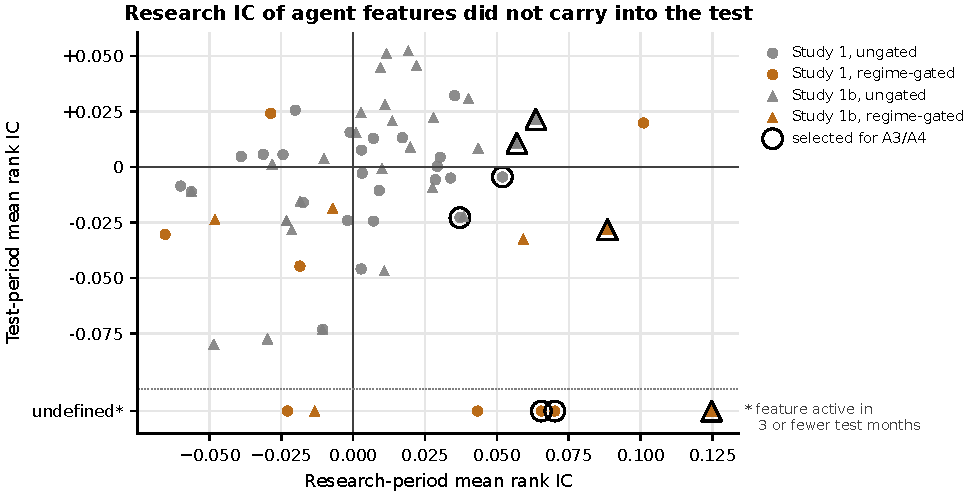
\includegraphics[width=\linewidth]{../report/figures/fig_agents_scatter.pdf}\caption{Research IC of agent features barely predicts their test IC; the selected regime-gated features were active in 3 test months. \textcolor{mute}{\footnotesize Source: analysis/\allowbreak{}output/\allowbreak{}study1/\allowbreak{}tables/\allowbreak{}d7\_\allowbreak{}agent\_\allowbreak{}candidates.csv.} \hfill \tagp}\end{figure}
\begin{figure}[H]\centering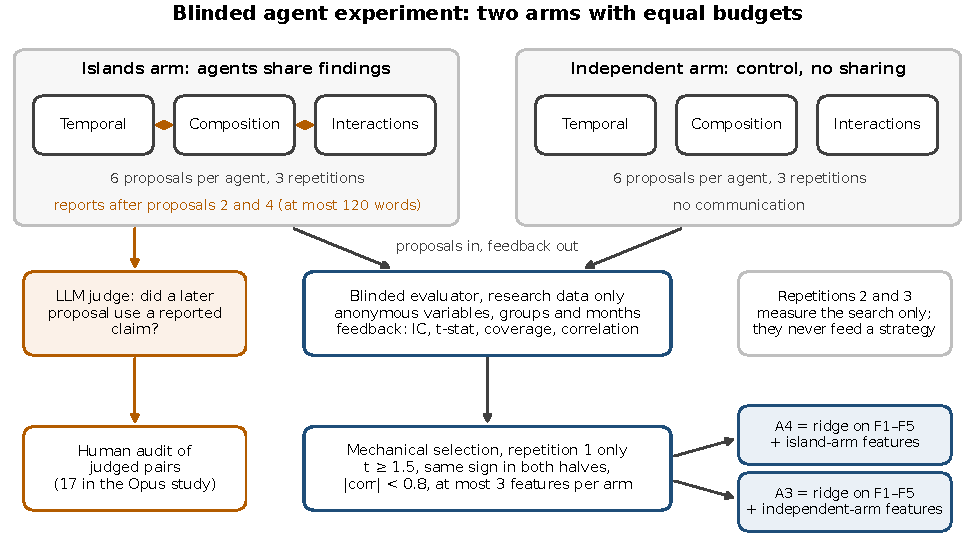
\includegraphics[width=\linewidth]{../report/figures/fig_agents.pdf}\caption{Two arms with equal budgets, a blinded evaluator, mechanical selection and a human-audited LLM judge. \textcolor{mute}{\footnotesize Source: frozen params.py AGENT.} \hfill \tagc}\end{figure}
\begin{figure}[H]\centering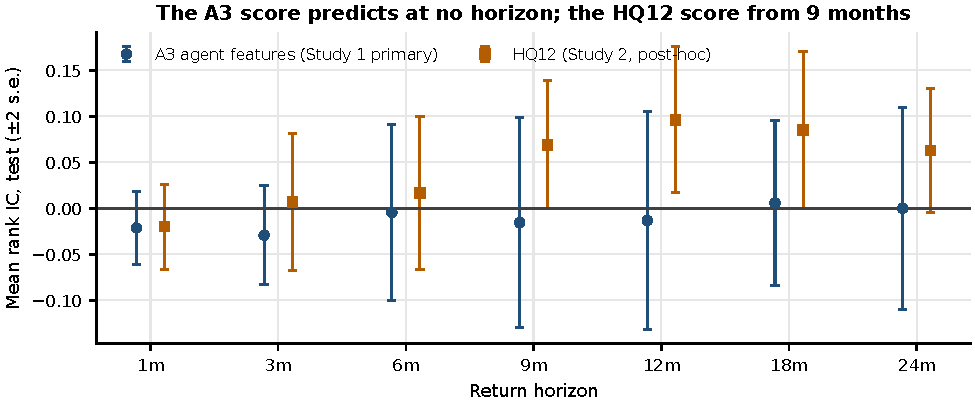
\includegraphics[width=\linewidth]{../report/figures/fig_s1_horizon.pdf}\caption{The A3 score has no IC at any horizon from 1 to 24 months; the HQ12 score has one from 9 months. \textcolor{mute}{\footnotesize Source: analysis/\allowbreak{}output/\allowbreak{}study1/\allowbreak{}tables/\allowbreak{}d11\_\allowbreak{}a3\_\allowbreak{}horizon\_\allowbreak{}profile.csv.} \hfill \tagp}\end{figure}
\begin{figure}[H]\centering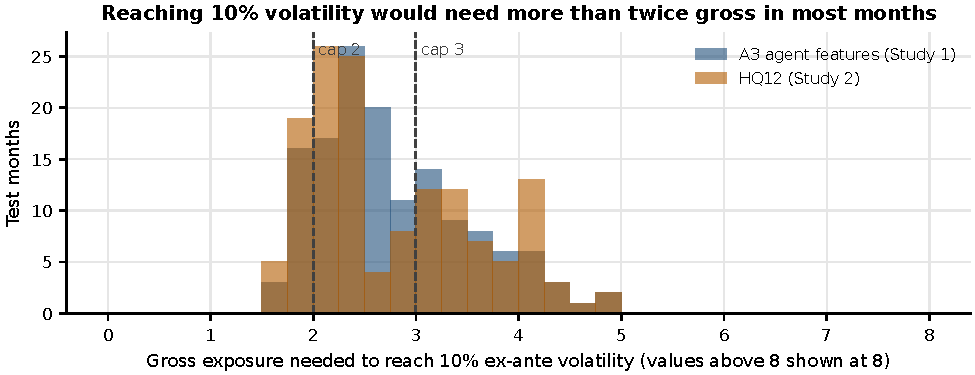
\includegraphics[width=\linewidth]{../report/figures/fig_s23_gross_needed.pdf}\caption{Reaching the 10\% volatility target would need a gross exposure above 2 in most test months, so the cap binds; the cap explains the volatility shortfall, not the losses. \textcolor{mute}{\footnotesize Source: analysis/\allowbreak{}output/\allowbreak{}study2/\allowbreak{}tables/\allowbreak{}s23\_\allowbreak{}r2\_\allowbreak{}distribution.csv.} \hfill \tagp}\end{figure}
\begin{figure}[H]\centering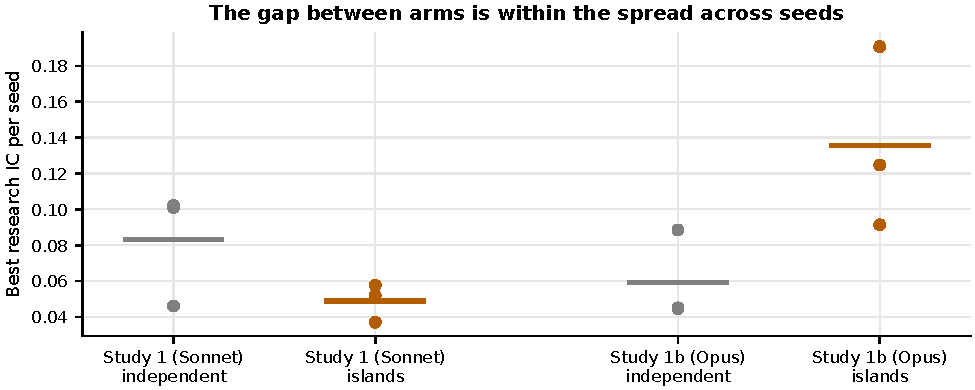
\includegraphics[width=\linewidth]{../report/figures/fig_s23_agents_seeds.pdf}\caption{Best research IC per seed, by study and arm: the gap between arms is within the spread across seeds. \textcolor{mute}{\footnotesize Source: analysis/\allowbreak{}output/\allowbreak{}study2/\allowbreak{}tables/\allowbreak{}s23\_\allowbreak{}r4\_\allowbreak{}agents\_\allowbreak{}by\_\allowbreak{}seed.csv.} \hfill \tagp}\end{figure}
\begin{figure}[H]\centering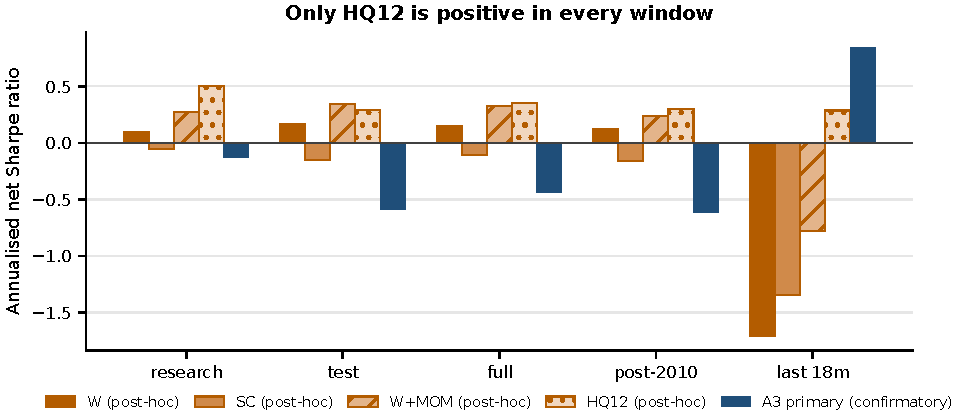
\includegraphics[width=\linewidth]{../report/figures/fig_v2_windows.pdf}\caption{HQ12 is the only variant positive in every window; W and W+MOM lost heavily in the last 18 months. \textcolor{mute}{\footnotesize Source: analysis/\allowbreak{}output/\allowbreak{}study2/\allowbreak{}tables/\allowbreak{}v2\_\allowbreak{}window\_\allowbreak{}stats.csv.} \hfill \tagp / \tagc (A3 bars)}\end{figure}
\clearpage\section{Statistics}
Each table lives in \path{analysis/output/study2/tables/<name>.csv}; the LaTeX fragment in \path{report/tables/<name>.tex}.
\subsection*{D1 single-signal rank IC \hfill \tagp}
{\footnotesize\setlength{\tabcolsep}{4pt}% POST-HOC | source: analysis/output/study1/tables/d1_signal_ic.csv (generated by analysis/run.ipynb)
\begin{tabular}{lrrr}
\toprule
Signal & Research 2004--14 & Test 2014--26 & Full 2004--26 \\
\midrule
F1 openings & +0.001 (+0.02) & $-$0.011 ($-$0.44) & $-$0.005 ($-$0.30) \\
F2 hires & +0.012 (+0.48) & +0.013 (+0.48) & +0.013 (+0.71) \\
F3 quits & +0.014 (+0.49) & +0.002 (+0.11) & +0.009 (+0.50) \\
F4 layoffs & +0.033 (+1.07) & +0.026 (+0.93) & +0.028 (+1.38) \\
F5 hours & $-$0.012 ($-$0.55) & $-$0.007 ($-$0.34) & $-$0.010 ($-$0.67) \\
W wage growth & +0.029 (+1.54) & +0.049 (+2.04) & +0.039 (+2.50) \\
A0 composite (prereg.) & $-$0.023 ($-$0.88) & $-$0.006 ($-$0.21) & $-$0.013 ($-$0.69) \\
Industry momentum 12-1 & +0.036 (+1.25) & +0.003 (+0.11) & +0.020 (+0.99) \\
\bottomrule
\end{tabular}
}\par
\medskip
\subsection*{D2 IC by horizon \hfill \tagp}
{\footnotesize\setlength{\tabcolsep}{4pt}% POST-HOC | source: analysis/output/study1/tables/d2_horizon_ic.csv (generated by analysis/run.ipynb)
\begin{tabular}{lrrrr}
\toprule
Signal & 1m & 3m & 6m & 12m \\
\midrule
F1 openings & $-$0.005 ($-$0.31) & +0.007 (+0.23) & $-$0.011 ($-$0.28) & $-$0.039 ($-$0.92) \\
F2 hires & +0.013 (+0.70) & +0.002 (+0.07) & +0.002 (+0.08) & $-$0.062 ($-$2.08) \\
F3 quits & +0.009 (+0.50) & $-$0.013 ($-$0.55) & $-$0.022 ($-$0.78) & $-$0.065 ($-$1.73) \\
F4 layoffs & +0.028 (+1.37) & +0.005 (+0.17) & +0.000 (+0.01) & $-$0.036 ($-$1.28) \\
F5 hours & $-$0.010 ($-$0.67) & $-$0.027 ($-$1.24) & $-$0.049 ($-$1.69) & $-$0.057 ($-$1.86) \\
W wage growth & +0.039 (+2.51) & +0.037 (+1.77) & +0.037 (+1.28) & +0.026 (+0.63) \\
A0 composite (prereg.) & $-$0.013 ($-$0.69) & $-$0.002 ($-$0.09) & $-$0.021 ($-$0.61) & $-$0.053 ($-$1.58) \\
Industry momentum 12-1 & +0.020 (+0.99) & +0.025 (+0.80) & +0.048 (+1.24) & +0.029 (+0.63) \\
\bottomrule
\end{tabular}
}\par
\medskip
\subsection*{D3a tightness regime balance \hfill \tagp}
{\footnotesize\setlength{\tabcolsep}{4pt}% POST-HOC | source: analysis/output/tables/d3_regime_balance.csv (generated by analysis/run.ipynb)
\begin{tabular}{lrr}
\toprule
Months in regime & Research 2004--14 & Test 2014--26 \\
\midrule
months & 125 & 142 \\
expanding low & 49 & 3 \\
expanding middle & 26 & 6 \\
expanding high & 50 & 133 \\
T rising (12m) & 93 & 88 \\
T falling (12m) & 32 & 54 \\
V/U > 1 & 0 & 75 \\
T min & $-$1.88 & $-$1.61 \\
T max & $-$0.30 & +0.71 \\
\bottomrule
\end{tabular}
}\par
\medskip
\subsection*{D3b IC when T rises vs falls \hfill \tagp}
{\footnotesize\setlength{\tabcolsep}{4pt}% POST-HOC | source: analysis/output/tables/d3_tightness_ic.csv (generated by analysis/run.ipynb)
\begin{tabular}{lrrr}
\toprule
Signal & T rising (182 m) & T falling (86 m) & Difference \\
\midrule
F1 openings & +0.001 (+0.05) & $-$0.019 ($-$0.47) & +0.019 \\
F2 hires & +0.032 (+1.51) & $-$0.026 ($-$0.74) & +0.059 \\
F3 quits & +0.024 (+1.32) & $-$0.024 ($-$0.76) & +0.048 \\
F4 layoffs & +0.013 (+0.53) & +0.060 (+1.69) & $-$0.046 \\
F5 hours & $-$0.002 ($-$0.13) & $-$0.026 ($-$1.00) & +0.024 \\
W wage growth & +0.033 (+1.67) & +0.053 (+2.04) & $-$0.020 \\
A0 composite (prereg.) & +0.003 (+0.13) & $-$0.045 ($-$1.28) & +0.048 \\
Industry momentum 12-1 & +0.036 (+1.68) & $-$0.014 ($-$0.33) & +0.050 \\
\bottomrule
\end{tabular}
}\par
\medskip
\subsection*{D4 test-period performance \hfill \tagc (A0-A4) / \tagp (momentum)}
{\footnotesize\setlength{\tabcolsep}{4pt}% CONFIRMATORY (A0-A4) / POST-HOC (momentum) | source: analysis/output/study1/tables/d4_test_performance.csv (generated by analysis/run.ipynb)
\begin{tabular}{lrrrrrr}
\toprule
strategy & Sharpe & Net p.a. & Vol. & Max DD & Turnover & Costs p.a. \\
\midrule
A0 fixed rule & $-$0.36 & $-$3.5\% & 9.7\% & $-$40.3\% & 0.83 & 1.01\% \\
A1 ridge & $-$0.51 & $-$4.0\% & 7.9\% & $-$37.7\% & 0.91 & 1.11\% \\
A3 primary & $-$0.58 & $-$4.6\% & 7.8\% & $-$41.1\% & 0.91 & 1.11\% \\
A4 island agents & $-$0.79 & $-$6.1\% & 7.8\% & $-$53.3\% & 1.11 & 1.35\% \\
Industry momentum 12-1 & +0.03 & +0.3\% & 9.4\% & $-$20.8\% & 0.53 & 0.65\% \\
\bottomrule
\end{tabular}
}\par
\medskip
\subsection*{D5 A3 P\&L by industry \hfill \tagp}
{\footnotesize\setlength{\tabcolsep}{4pt}% POST-HOC | source: analysis/output/study1/tables/d5_industry_pnl.csv (generated by analysis/run.ipynb)
\begin{tabular}{lrrr}
\toprule
component & Contribution (pp) & Months long & Months short \\
\midrule
Mining \& logging & +7.2 & 33\% & 36\% \\
Construction & $-$19.2 & 36\% & 39\% \\
Durable mfg & +1.8 & 31\% & 24\% \\
Nondurable mfg & +5.4 & 32\% & 35\% \\
Wholesale & +14.9 & 31\% & 42\% \\
Retail & +0.2 & 39\% & 35\% \\
Transport \& utilities & +1.4 & 47\% & 30\% \\
Information & $-$5.8 & 30\% & 37\% \\
Finance \& insurance & $-$16.3 & 34\% & 45\% \\
Real estate & $-$1.6 & 24\% & 45\% \\
Prof. \& business svcs & $-$12.2 & 18\% & 47\% \\
Health care & $-$26.2 & 41\% & 36\% \\
Accommodation \& food & +4.5 & 46\% & 22\% \\
Market hedge & +4.6 &  &  \\
Trading costs & $-$13.1 &  &  \\
\bottomrule
\end{tabular}
}\par
\medskip
\subsection*{D6 factor loadings \hfill \tagc}
{\footnotesize\setlength{\tabcolsep}{4pt}% CONFIRMATORY | source: analysis/output/study1/tables/d6_factor_loadings.csv (generated by analysis/run.ipynb)
\begin{tabular}{lrrr}
\toprule
Factor & A0 fixed rule & A1 ridge & A3 primary \\
\midrule
Alpha (per month) & $-$0.25\% ($-$0.92) & $-$0.35\% ($-$1.72) & $-$0.38\% ($-$1.86) \\
Market & $-$0.01 ($-$0.31) & $-$0.01 ($-$0.20) & $-$0.03 ($-$0.43) \\
SMB & +0.02 (+0.21) & +0.12 (+1.01) & +0.10 (+0.89) \\
HML & +0.09 (+0.60) & $-$0.15 ($-$1.97) & $-$0.15 ($-$2.01) \\
RMW & +0.00 (+0.05) & +0.21 (+2.33) & +0.19 (+2.16) \\
CMA & $-$0.04 ($-$0.21) & +0.05 (+0.47) & +0.03 (+0.26) \\
Momentum & $-$0.06 ($-$0.72) & +0.01 (+0.15) & $-$0.01 ($-$0.17) \\
Industry momentum & +0.22 (+1.93) & $-$0.02 ($-$0.21) & $-$0.01 ($-$0.12) \\
\bottomrule
\end{tabular}
}\par
\medskip
\subsection*{D7a agent candidates \hfill \tagp}
{\footnotesize\setlength{\tabcolsep}{4pt}% POST-HOC | source: analysis/output/tables/d7_agent_summary.csv (generated by analysis/run.ipynb)
\begin{tabular}{lrr}
\toprule
Repetition-1 candidates & Sonnet & Opus \\
\midrule
valid candidates & 33.0 & 35.0 \\
regime-gated & 9.0 & 6.0 \\
test IC undefined ($\leq$3 active months) & 4.0 & 2.0 \\
corr(research IC, test IC) & 0.22 & 0.37 \\
passed research filter & 4.0 & 7.0 \\
selected & 4.0 & 4.0 \\
selected and regime-gated & 2.0 & 2.0 \\
selected with positive test IC & 0.0 & 2.0 \\
\bottomrule
\end{tabular}
}\par
\medskip
\subsection*{D7b selected agent features \hfill \tagp}
{\footnotesize\setlength{\tabcolsep}{4pt}% POST-HOC | source: analysis/output/study1/tables/d7_selected_features.csv (generated by analysis/run.ipynb)
\begin{tabular}{llp{2.55in}rr}
\toprule
Study & Arm & Feature (decoded) & Research IC (n) & Test IC (n) \\
\midrule
Study 1 & independent & regime(yoy(Earnings), "low") & +0.065 (48) & n/a (3) \\
Study 1 & independent & regime(spread(tsz(Layoffs, 60), tsz(Hires, 60)), "low") & +0.070 (43) & n/a (3) \\
Study 1 & communicating & spread(chg(Layoffs, 3), chg(Openings, 3)) & +0.037 (123) & $-$0.023 (142) \\
Study 1 & communicating & spread(chg(Layoffs, 6), chg(Openings, 6)) & +0.052 (120) & $-$0.004 (142) \\
Study 1b & independent & mult(regime(tsz(Hires, "exp"), "high"), csrank(tsz(Openings, "exp"))) & +0.088 (15) & $-$0.028 (133) \\
Study 1b & communicating & tsz(lchg(lag(Earnings, 1), 12), 36) & +0.064 (78) & +0.022 (142) \\
Study 1b & communicating & regime(spread(chg(Quits, 3), chg(Hires, 3)), "low") & +0.125 (48) & n/a (3) \\
Study 1b & communicating & tsz(lchg(lag(Hours, 1), 12), 36) & +0.057 (78) & +0.011 (142) \\
\bottomrule
\end{tabular}
}\par
\medskip
\subsection*{D8 A3 by window \hfill \tagc}
{\footnotesize\setlength{\tabcolsep}{4pt}% CONFIRMATORY | source: analysis/output/tables/d8_a3_windows.csv (generated by analysis/run.ipynb)
\begin{tabular}{lrrrr}
\toprule
window & Months & Sharpe & Net return p.a. & Mean IC (t) \\
\midrule
Full test, Nov 2014-Aug 2026 & 142 & $-$0.58 & $-$4.6\% & $-$0.021 ($-$1.08) \\
First half & 71 & $-$0.72 & $-$4.9\% & $-$0.028 ($-$0.90) \\
Second half & 71 & $-$0.49 & $-$4.3\% & $-$0.015 ($-$0.59) \\
Excluding Mar-Dec 2020 & 132 & $-$0.51 & $-$4.1\% & $-$0.012 ($-$0.56) \\
Last 18 months (Mar 2025-Aug 2026) & 18 & +0.85 & +6.7\% & +0.033 (+0.44) \\
Course window "full" (from Jun 2007) & 231 & $-$0.44 & $-$3.2\% & $-$0.009 ($-$0.49) \\
Course window "post-2010" & 200 & $-$0.62 & $-$4.4\% & $-$0.019 ($-$1.02) \\
\bottomrule
\end{tabular}
}\par
\medskip
\subsection*{D9 risk overlay \hfill \tagp}
{\footnotesize\setlength{\tabcolsep}{4pt}% POST-HOC | source: analysis/output/study1/tables/d9_risk_overlay.csv (generated by analysis/run.ipynb)
\begin{tabular}{lrrrrr}
\toprule
Study, strategy & Cap binds & Ex-ante vol & Realised vol & Gross leverage & |Hedge| \\
\midrule
Study 1 A0 & 80\% & 8.0\% & 9.7\% & 1.96 & 0.15 \\
Study 1 A1 & 88\% & 7.5\% & 7.9\% & 1.98 & 0.13 \\
Study 1 A1-T & 82\% & 7.5\% & 8.2\% & 1.97 & 0.12 \\
Study 1 A3 & 87\% & 7.5\% & 7.8\% & 1.98 & 0.13 \\
Study 1 A4 & 91\% & 7.3\% & 7.8\% & 1.99 & 0.13 \\
Study 1b A3 & 92\% & 7.3\% & 7.5\% & 1.99 & 0.15 \\
Study 1b A4 & 93\% & 7.3\% & 8.4\% & 1.99 & 0.11 \\
\bottomrule
\end{tabular}
}\par
\medskip
\subsection*{D10 agent experiment design \hfill \tagc}
{\footnotesize\setlength{\tabcolsep}{4pt}% CONFIRMATORY | source: analysis/output/study1/tables/d10_agent_design.csv (generated by analysis/run.ipynb)
\begin{tabular}{llp{3.3in}}
\toprule
study & item & value \\
\midrule
Both & Arms & islands (communicating), independent (control) \\
Both & Agents per arm & Temporal, Composition, Interactions \\
Both & Proposals per agent x repetitions & 6 x 3 \\
Both & Migration reports & after proposals 2 and 4, at most 120 words \\
Both & Selection (repetition 1 only) & t $\geq$ 1.5, same sign in both halves, |corr| < 0.8, at most 3 per arm \\
Sonnet & Valid proposals & 98 / 108 \\
Sonnet & Migration reports admitted & 7 / 18 \\
Sonnet & Defined LLM-judge uptake labels & 8 / 36 \\
Sonnet & Human-audited judge pairs & 8 \\
Opus & Valid proposals & 106 / 108 \\
Opus & Migration reports admitted & 15 / 18 \\
Opus & Defined LLM-judge uptake labels & 84 / 88 \\
Opus & Human-audited judge pairs & 17 \\
Opus & Human-judge agreement & 10 / 17 (human yes 3, judge yes 10) \\
\bottomrule
\end{tabular}
}\par
\medskip
\subsection*{v2 variants: Sharpe by window and test statistics \hfill \tagp}
{\footnotesize\setlength{\tabcolsep}{4pt}% POST-HOC | source: analysis/output/tables/v2_results.csv (generated by analysis/run.ipynb)
\begin{tabular}{lrrrrrrrrr}
\toprule
Variant & Research & Test & Full & Post-2010 & Last 18m & Test IC (t) & Alpha t & Placebo p & DSR \\
\midrule
V2a & +0.09 & +0.16 & +0.15 & +0.12 & $-$1.71 & +0.049 (+2.04) & +0.29 & 0.02 & 0.02 \\
V2b & $-$0.06 & $-$0.15 & $-$0.11 & $-$0.16 & $-$1.34 & +0.042 (+1.65) & $-$0.84 & 0.05 & 0.00 \\
V2c & +0.27 & +0.35 & +0.32 & +0.24 & $-$0.78 & +0.032 (+1.21) & +1.36 & 0.26 & 0.09 \\
V2d & +0.50 & +0.29 & +0.35 & +0.30 & +0.29 & $-$0.020 ($-$0.87) & +1.37 & 0.85 & 0.06 \\
\bottomrule
\end{tabular}
}\par
\medskip
\clearpage\section{HQ12 robustness battery (v3)}
Spec \path{analysis/specs/study2_2_hq12_robustness.md} frozen 2026-10-03T09:52:27Z, first run 09:53:32Z; every check run once; $N_{\text{trials}}$ raised to 132. Results: \path{analysis/output/study2/v3_results.md}. \hfill \tagp

\emph{Reading against the pre-declared rule: fragile in one dimension (R4).} HQ12 lost money in the first half of the test (Sharpe $-0.21$) and made it in the second ($+0.64$); the other six conditions hold. The 12-month IC is positive in both halves.

\subsection*{R1 Components \hfill \tagp}
{\footnotesize\setlength{\tabcolsep}{4pt}% POST-HOC | source: analysis/output/study2/tables/v3_r1_components.csv (generated by analysis/run.ipynb)
\begin{tabular}{lrrrrr}
\toprule
Sharpe research & Sharpe test & Sharpe full & Test IC 12m (t) & Test alpha t \\
\midrule
+0.41 & +0.19 & +0.27 & +0.093 (+2.90) & +0.79 \\
+0.18 & +0.16 & +0.15 & +0.085 (+1.75) & +0.81 \\
+0.10 & +0.42 & +0.29 & +0.082 (+1.38) & +1.48 \\
+0.11 & +0.16 & +0.13 & +0.032 (+0.87) & +0.69 \\
+0.50 & +0.29 & +0.35 & +0.096 (+2.43) & +1.37 \\
\bottomrule
\end{tabular}
}\par\medskip
\subsection*{R2 Horizon profile \hfill \tagp}
\begin{figure}[H]\centering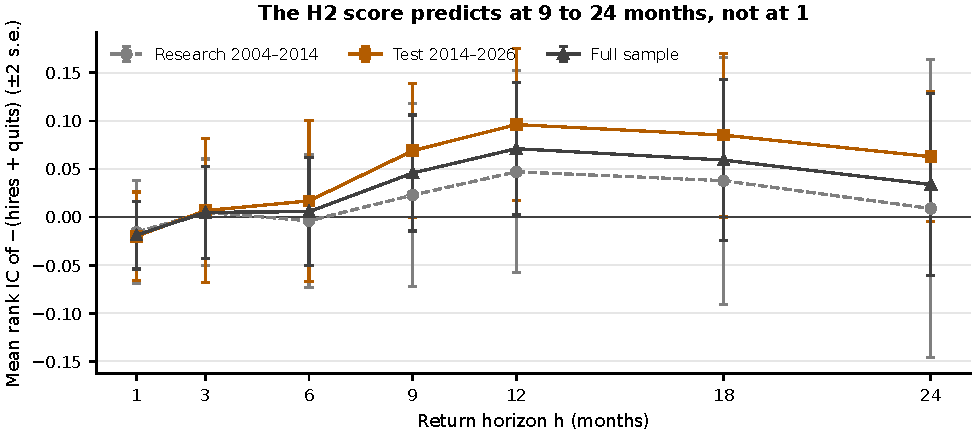
\includegraphics[width=\linewidth]{../report/figures/fig_horizon_profile.pdf}
\caption{The HQ12 score has no one-month IC and a positive IC from 9 to 24 months, peaking at 12 (test $+0.096$, $t=2.43$). \textcolor{mute}{\footnotesize Source: analysis/output/study2/tables/v3\_r2\_horizon\_profile.csv.} \hfill \tagp}\end{figure}
{\footnotesize\setlength{\tabcolsep}{4pt}% POST-HOC | source: analysis/output/study2/tables/v3_r2_horizon_profile.csv (generated by analysis/run.ipynb)
\begin{tabular}{lrrr}
\toprule
research & test & full \\
\midrule
$-$0.016 ($-$0.59) & $-$0.020 ($-$0.87) & $-$0.019 ($-$1.08) \\
+0.005 (+0.18) & +0.007 (+0.18) & +0.005 (+0.21) \\
$-$0.004 ($-$0.11) & +0.017 (+0.40) & +0.006 (+0.20) \\
+0.023 (+0.48) & +0.069 (+1.98) & +0.046 (+1.52) \\
+0.047 (+0.90) & +0.096 (+2.43) & +0.071 (+2.06) \\
+0.038 (+0.59) & +0.085 (+2.00) & +0.059 (+1.41) \\
+0.009 (+0.11) & +0.063 (+1.86) & +0.034 (+0.72) \\
\bottomrule
\end{tabular}
}\par\medskip
\subsection*{R3 Holding period \hfill \tagp}
\begin{figure}[H]\centering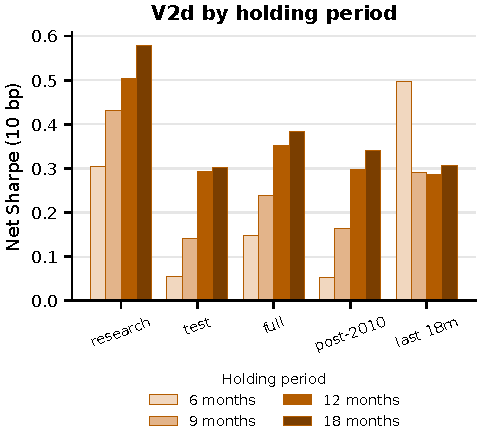
\includegraphics[width=0.55\linewidth]{../report/figures/fig_v2d_holding.pdf}
\caption{Longer holding helps: test Sharpe $+0.05$ at 6 months, $+0.29$ at 12, $+0.30$ at 18. \textcolor{mute}{\footnotesize Source: v3\_r3\_holding.csv.} \hfill \tagp}\end{figure}
{\footnotesize\setlength{\tabcolsep}{4pt}% POST-HOC | source: analysis/output/study2/tables/v3_r3_holding.csv (generated by analysis/run.ipynb)
\begin{tabular}{lrrrrrr}
\toprule
Holding & research & test & full & post-2010 & last 18m & Test turnover \\
\midrule
6 months & +0.31 & +0.05 & +0.15 & +0.05 & +0.50 & 0.49 \\
9 months & +0.43 & +0.14 & +0.24 & +0.16 & +0.29 & 0.40 \\
12 months & +0.50 & +0.29 & +0.35 & +0.30 & +0.29 & 0.37 \\
18 months & +0.58 & +0.30 & +0.38 & +0.34 & +0.31 & 0.28 \\
\bottomrule
\end{tabular}
}\par\medskip
\subsection*{R4 Sub-periods \hfill \tagp}
{\footnotesize\setlength{\tabcolsep}{4pt}% POST-HOC | source: analysis/output/tables/v3_r4_subperiods.csv (generated by analysis/run.ipynb)
\begin{tabular}{lrrrr}
\toprule
Window & Months & Sharpe & Net p.a. & IC 12m (t) \\
\midrule
test: first half & 71 & $-$0.21 & $-$1.4\% & +0.097 (+1.75) \\
test: second half & 71 & +0.64 & +6.5\% & +0.095 (+1.60) \\
test: excl. Mar 2020-Dec 2021 & 120 & +0.37 & +3.0\% & +0.105 (+2.23) \\
test: pre-2020 & 62 & +0.14 & +0.8\% & +0.114 (+1.92) \\
test: 2020 onward & 80 & +0.37 & +3.9\% & +0.080 (+1.54) \\
full: first half & 134 & +0.33 & +2.0\% & +0.038 (+0.73) \\
full: second half & 134 & +0.38 & +3.3\% & +0.107 (+2.66) \\
full: excl. Mar 2020-Dec 2021 & 246 & +0.40 & +2.9\% & +0.073 (+1.93) \\
full: pre-2020 & 188 & +0.36 & +2.2\% & +0.068 (+1.57) \\
\bottomrule
\end{tabular}
}\par\medskip
\subsection*{R5 Costs \hfill \tagp}
{\footnotesize\setlength{\tabcolsep}{4pt}% POST-HOC | source: analysis/output/study2/tables/v3_r5_costs.csv (generated by analysis/run.ipynb)
\begin{tabular}{lrrrrr}
\toprule
Window & 0 bp & 10 bp & 25 bp & 50 bp & Break-even (bp) \\
\midrule
research & +0.58 & +0.50 & +0.39 & +0.20 & 76 \\
test & +0.34 & +0.29 & +0.22 & +0.09 & 68 \\
full & +0.41 & +0.35 & +0.26 & +0.11 & 69 \\
post-2010 & +0.35 & +0.30 & +0.21 & +0.07 & 63 \\
last 18m & +0.32 & +0.29 & +0.24 & +0.16 & 99 \\
\bottomrule
\end{tabular}
}\par\medskip
\subsection*{R6 Factor regression, 12 HAC lags \hfill \tagp}
{\footnotesize\setlength{\tabcolsep}{4pt}% POST-HOC | source: analysis/output/study2/tables/v3_r6_alpha.csv (generated by analysis/run.ipynb)
\begin{tabular}{lrr}
\toprule
Test (HAC 12) & Full (HAC 12) \\
\midrule
+0.26\% (+1.48) & +0.26\% (+1.92) \\
+0.03 (+0.58) & $-$0.00 ($-$0.08) \\
$-$0.17 ($-$2.24) & $-$0.02 ($-$0.31) \\
+0.12 (+1.07) & +0.10 (+1.23) \\
$-$0.36 ($-$4.45) & $-$0.16 ($-$1.83) \\
$-$0.01 ($-$0.07) & $-$0.09 ($-$0.87) \\
$-$0.12 ($-$1.14) & $-$0.03 ($-$0.51) \\
+0.02 (+0.17) & +0.06 (+0.93) \\
\bottomrule
\end{tabular}
}\par\medskip
\subsection*{R7 Drop one industry \hfill \tagp}
\begin{figure}[H]\centering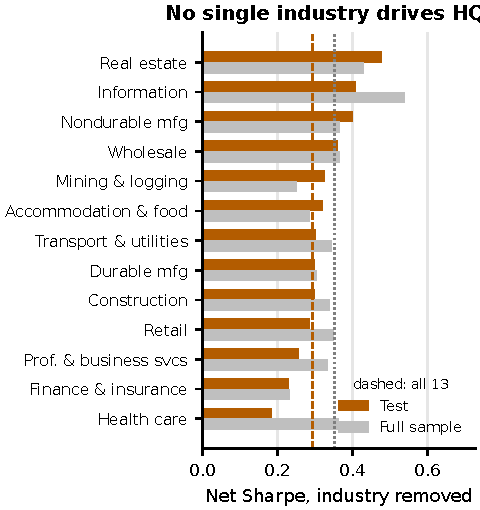
\includegraphics[width=0.55\linewidth]{../report/figures/fig_v2d_dropone.pdf}
\caption{No single industry carries HQ12: removing any one leaves the test Sharpe between $+0.18$ and $+0.48$. \textcolor{mute}{\footnotesize Source: v3\_r7\_dropone.csv.} \hfill \tagp}\end{figure}
{\footnotesize\setlength{\tabcolsep}{4pt}% POST-HOC | source: analysis/output/study2/tables/v3_r7_dropone_summary.csv (generated by analysis/run.ipynb)
\begin{tabular}{lrr}
\toprule
statistic & Test Sharpe & Full Sharpe \\
\midrule
minimum & +0.18 & +0.23 \\
median & +0.30 & +0.34 \\
maximum & +0.48 & +0.54 \\
all 13 groups (HQ12) & +0.29 & +0.35 \\
industry whose removal lowers test Sharpe most & Health care &  \\
industry whose removal raises test Sharpe most & Real estate &  \\
\bottomrule
\end{tabular}
}\par\medskip
\subsection*{R8 Tightness moderator \hfill \tagp}
\begin{figure}[H]\centering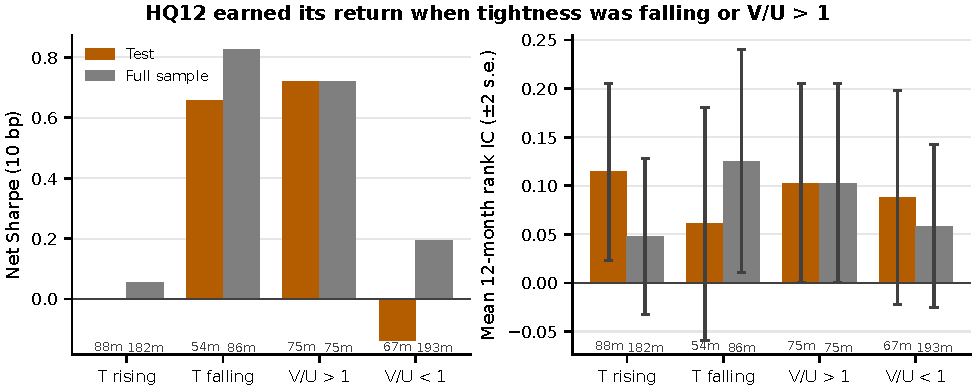
\includegraphics[width=\linewidth]{../report/figures/fig_v2d_tightness.pdf}
\caption{HQ12 earned its return when tightness was falling or $V/U>1$; in tightening months the Sharpe was zero although the 12-month IC was highest. \textcolor{mute}{\footnotesize Source: v3\_r8\_tightness.csv.} \hfill \tagp}\end{figure}
{\footnotesize\setlength{\tabcolsep}{4pt}% POST-HOC | source: analysis/output/study2/tables/v3_r8_tightness.csv (generated by analysis/run.ipynb)
\begin{tabular}{lrrrr}
\toprule
Months & Sharpe & Net p.a. & IC 12m (t) \\
\midrule
88 & $-$0.00 & $-$0.0\% & +0.115 (+2.52) \\
54 & +0.66 & +6.8\% & +0.061 (+1.02) \\
75 & +0.72 & +6.0\% & +0.103 (+2.00) \\
67 & $-$0.14 & $-$1.2\% & +0.088 (+1.59) \\
182 & +0.06 & +0.4\% & +0.048 (+1.19) \\
86 & +0.83 & +7.6\% & +0.126 (+2.19) \\
75 & +0.72 & +6.0\% & +0.103 (+2.00) \\
193 & +0.19 & +1.4\% & +0.059 (+1.40) \\
\bottomrule
\end{tabular}
}\par\medskip
\subsection*{R9 Block-bootstrap interval \hfill \tagp}
{\footnotesize\setlength{\tabcolsep}{4pt}% POST-HOC | source: analysis/output/tables/v3_r9_bootstrap.csv (generated by analysis/run.ipynb)
\begin{tabular}{lrrrr}
\toprule
Window & Sharpe & 90\% interval & Months & Excludes 0 \\
\midrule
test & +0.29 & [$-$0.07, +0.65] & 142 & no \\
full & +0.35 & [+0.05, +0.64] & 268 & yes \\
\bottomrule
\end{tabular}
}\par\medskip
\subsection*{R10 As-known data \hfill \tagp}
{\footnotesize\setlength{\tabcolsep}{4pt}% POST-HOC | source: analysis/output/tables/v3_r10_asknown.csv (generated by analysis/run.ipynb)
\begin{tabular}{p{4.2cm}p{2.6cm}p{8.6cm}}
\toprule
check & status & note \\
\midrule
R10 as-known (ALFRED vintage) rerun of V2a-V2d & not run: no key & analysis/.env has no FRED\_API\_KEY; historical v2/v3 results use revised data with fixed lags (data\_vintage.md) \\
\bottomrule
\end{tabular}
}\par\medskip
\subsection*{R11 Fundamental law, test window \hfill \tagc\ (A3) / \tagp}
{\footnotesize\setlength{\tabcolsep}{4pt}% CONFIRMATORY (A3) / POST-HOC | source: analysis/output/tables/v3_r11_fundamental_law.csv (generated by analysis/run.ipynb)
\begin{tabular}{lrrrrrrr}
\toprule
Book (test window) & IC & Horizon & BR/yr & TC & Implied IR & Ceiling (TC=1) & Realised Sharpe \\
\midrule
A3 primary & $-$0.021 & 1m & 156 & 0.80 & $-$0.21 & $-$0.27 & $-$0.58 \\
V2a wage growth & +0.049 & 1m & 156 & 0.91 & +0.56 & +0.62 & +0.16 \\
V2d -(hires+quits) 12m & +0.096 & 12m & 13 & 0.48 & +0.17 & +0.35 & +0.29 \\
\bottomrule
\end{tabular}
}\par\medskip
\subsection*{Deflated Sharpe at 112 and 132 trials \hfill \tagp}
{\footnotesize\setlength{\tabcolsep}{4pt}% POST-HOC | source: analysis/output/study2/tables/v3_dsr132.csv (generated by analysis/run.ipynb)
\begin{tabular}{llrrr}
\toprule
Window & DSR (112 trials) & DSR (132 trials) & Benchmark Sharpe (132) \\
\midrule
test & 0.02 & 0.02 & 0.76 \\
full & 0.03 & 0.03 & 0.56 \\
test & 0.00 & 0.00 & 0.76 \\
full & 0.00 & 0.00 & 0.56 \\
test & 0.09 & 0.08 & 0.76 \\
full & 0.16 & 0.15 & 0.56 \\
test & 0.06 & 0.05 & 0.76 \\
full & 0.18 & 0.16 & 0.56 \\
\bottomrule
\end{tabular}
}\par\medskip
\subsection*{Reading rule \hfill \tagp}
{\footnotesize\setlength{\tabcolsep}{4pt}% POST-HOC | source: analysis/output/tables/v3_reading.csv (generated by analysis/run.ipynb)
\begin{tabular}{lr}
\toprule
condition & holds \\
\midrule
R1 hires-only and quits-only test Sharpe > 0 & yes \\
R2 test 12m IC t >= 2 and 1m IC t < 2 & yes \\
R3 holding 9 and 18 months test Sharpe > 0 & yes \\
R4 both test halves Sharpe > 0 & no \\
R5 test break-even cost > 25 bp & yes \\
R7 minimum drop-one test Sharpe > 0 & yes \\
R9 90\% interval excludes 0 (test or full) & yes \\
\bottomrule
\end{tabular}
}\par\medskip

\clearpage\section{Study 1 robustness and Study 2.3}
Study 1 rows labelled confirmatory are read from the saved results and are unchanged; everything else is post hoc (spec \path{analysis/specs/study2_3_robustness.md}, 162 looks). Sources: \path{analysis/output/study1/robustness.md} and \path{analysis/output/study2/robustness_2_3.md}.
\subsection*{Study 1: A3 and A0 \hfill \tagc\ / \tagp}
{\scriptsize\setlength{\tabcolsep}{3pt}% CONFIRMATORY / POST-HOC | source: analysis/output/study1/tables/d11_study1_robustness.csv (generated by analysis/run.ipynb)
\begin{tabular}{p{6.1cm}p{5.0cm}p{3.6cm}}
\toprule
Check (test window, as-known data unless stated) & A3 agent features (primary) & A0 fixed rule \\
\midrule
Test Sharpe, data as known & $-$0.58 & $-$0.36 \\
Test Sharpe, data first release & $-$0.52 & $-$0.16 \\
Test Sharpe, data revised & $-$0.56 & $-$0.26 \\
Test Sharpe, data fixed lag & $-$0.53 & $-$0.27 \\
Net return p.a. & $-$4.6\% & $-$3.5\% \\
IC, one month (t) & $-$0.021 ($-$1.08) & $-$0.020 ($-$0.71) \\
Factor alpha per month (t) & $-$0.38\% ($-$1.86) & $-$0.25\% ($-$0.92) \\
Placebo p (circular shift) & 0.72 & n/a (primary only) \\
Holm-adjusted p, IC and return & 1.00, 1.00 (A3 vs A1) & 1.00, 1.00 (A1 vs A0) \\
Deflated Sharpe, research (41 trials) & 0.003 & 0.000 \\
Sharpe at 0 / 10 / 25 bp & $-$0.45 / $-$0.58 / $-$0.79 & n/a / $-$0.36 / n/a \\
Sharpe, first test half & $-$0.72 & $-$0.55 \\
Sharpe, second test half & $-$0.49 & $-$0.20 \\
Sharpe, excluding Mar-Dec 2020 & $-$0.51 & $-$0.18 \\
Sharpe, last 18 months & +0.85 & $-$1.56 \\
Drop one group, Sharpe range & $-$0.70 (Wholesale) to $-$0.24 (Durable mfg) & n/a (primary only) \\
Gates G1 timing / G2 prediction / G3 alpha / G4 robustness / G5 implementable & pass / fail / fail / fail / fail & n/a (primary only) \\
Verdict & Do not implement & not primary \\
Block-bootstrap 90\% interval, test Sharpe & [$-$0.99, $-$0.16] & [$-$0.91, +0.20] \\
A3 score IC at 1 / 6 / 12 / 24 months (t) & $-$0.021 ($-$1.08) / $-$0.004 ($-$0.09) / $-$0.013 ($-$0.22) / $-$0.000 ($-$0.00) & n/a \\
A3 Sharpe with cap 2 / cap 3 / no cap & $-$0.58 / $-$0.61 / $-$0.62 & n/a \\
A3 Sharpe, rank-weighted book & $-$0.49 & n/a \\
\bottomrule
\end{tabular}
}\par\medskip
{\scriptsize\setlength{\tabcolsep}{3pt}% CONFIRMATORY | source: analysis/output/study1/tables/d11_freeze_check.csv (generated by analysis/run.ipynb)
\begin{tabular}{p{8cm}lp{6cm}}
\toprule
check & ok & value \\
\midrule
SHA-256 of FREEZE.json equals evaluation\_started.freeze\_sha256 & True & 60ea05294ffc856e \\
Freeze recorded (UTC) & True & 2026-10-02T06:00:09.537758+00:00 \\
Test opened (UTC) & True & 2026-10-02T06:00:09.578162+00:00 \\
Test opened after the freeze & True & 0.040 s later \\
Files in the freeze inventory & True & 525 \\
of which present in the repository & True & 338 \\
present files whose hash matches the inventory & True & 337 \\
present files that differ & True & outputs/human\_migration\_review.md \\
First test decision in the freeze record & True & 2014-10-31 \\
\bottomrule
\end{tabular}
}\par\medskip
{\footnotesize\setlength{\tabcolsep}{3pt}% POST-HOC | source: analysis/output/study1/tables/d11_a3_horizon_profile.csv (generated by analysis/run.ipynb)
\begin{tabular}{lrr}
\toprule
A3 agent features (Study 1 primary) & HQ12 (Study 2, post-hoc) \\
\midrule
$-$0.021 ($-$1.08) & $-$0.020 ($-$0.87) \\
$-$0.029 ($-$1.08) & +0.007 (+0.18) \\
$-$0.004 ($-$0.09) & +0.017 (+0.40) \\
$-$0.015 ($-$0.27) & +0.069 (+1.98) \\
$-$0.013 ($-$0.22) & +0.096 (+2.43) \\
+0.006 (+0.13) & +0.085 (+2.00) \\
$-$0.000 ($-$0.00) & +0.063 (+1.86) \\
\bottomrule
\end{tabular}
}\par\medskip
\subsection*{R1 As-known rerun \hfill \tagp}
{\footnotesize\setlength{\tabcolsep}{3pt}% POST-HOC | source: analysis/output/study2/tables/s23_r1_variants.csv (generated by analysis/run.ipynb)
\begin{tabular}{lrrrrrrr}
\toprule
Variant (test window) & Sharpe, fixed lag & Sharpe, as known & IC (t), fixed lag & IC (t), as known & Alpha t & Same top 3 & Same bottom 3 \\
\midrule
W & +0.16 & +0.13 & +0.049 (+2.04) & +0.041 (+1.73) & +0.18 & 76\% & 70\% \\
SC & $-$0.15 & +0.24 & +0.042 (+1.65) & +0.021 (+0.75) & +0.71 & 0\% & 0\% \\
W+MOM & +0.35 & +0.46 & +0.032 (+1.21) & +0.036 (+1.40) & +1.93 & 84\% & 74\% \\
HQ12 & +0.29 & +0.20 & +0.096 (+2.43) & +0.085 (+2.26) & +0.92 & 39\% & 51\% \\
\bottomrule
\end{tabular}
}\par\medskip
{\footnotesize\setlength{\tabcolsep}{3pt}% POST-HOC | source: analysis/output/study2/tables/s23_r1_hq12_battery.csv (generated by analysis/run.ipynb)
\begin{tabular}{lrr}
\toprule
HQ12 check & Fixed lag (Study 2.2) & As known (Study 2.3) \\
\midrule
Test Sharpe (10 bp) & +0.29 & +0.20 \\
Full-sample Sharpe (10 bp) & +0.35 & +0.31 \\
12-month IC, test & +0.10 & +0.08 \\
12-month IC t, test & +2.43 & +2.26 \\
1-month IC t, test & $-$0.87 & $-$0.42 \\
Component hires only, test Sharpe & +0.19 & +0.19 \\
Component quits only, test Sharpe & +0.16 & +0.17 \\
Holding 9 months, test Sharpe & +0.14 & +0.16 \\
Holding 18 months, test Sharpe & +0.30 & +0.11 \\
First test half, Sharpe & $-$0.21 & $-$0.23 \\
Second test half, Sharpe & +0.64 & +0.49 \\
Test Sharpe at 0 bp & +0.34 & +0.25 \\
Test Sharpe at 25 bp & +0.22 & +0.13 \\
Test Sharpe at 50 bp & +0.09 & $-$0.00 \\
Break-even cost, test (bp) & 68 & 50 \\
Drop one group, minimum test Sharpe & +0.18 & +0.05 \\
Drop one group, maximum test Sharpe & +0.48 & +0.36 \\
Bootstrap 90\% interval, test: low & $-$0.07 & $-$0.14 \\
Bootstrap 90\% interval, test: high & +0.65 & +0.57 \\
Alpha per month (\%), test, HAC 12 & +0.26 & +0.16 \\
Alpha t, test, HAC 12 & +1.48 & +0.92 \\
Bootstrap 90\% interval, full: low & +0.05 & +0.02 \\
Bootstrap 90\% interval, full: high & +0.64 & +0.60 \\
Alpha per month (\%), full, HAC 12 & +0.26 & +0.21 \\
Alpha t, full, HAC 12 & +1.92 & +1.81 \\
Deflated Sharpe, test (132 looks fixed lag; 162 as known) & +0.05 & +0.02 \\
\bottomrule
\end{tabular}
}\par\medskip
\subsection*{R2 Risk overlay and R3 rank-weighted books \hfill \tagp}
{\footnotesize\setlength{\tabcolsep}{3pt}% POST-HOC (diagnostic of a confirmatory book for A3) | source: analysis/output/study2/tables/s23_r2_risk_overlay.csv (generated by analysis/run.ipynb)
\begin{tabular}{llrrrrr}
\toprule
Book & Cap & Sharpe & Realised vol & Mean gross & Cap binds & Max drawdown \\
\midrule
A3 & 2 & $-$0.58 & 7.8\% & 1.98 & 87\% & $-$41.1\% \\
A3 & 3 & $-$0.61 & 9.7\% & 2.57 & 35\% & $-$50.7\% \\
A3 & none & $-$0.62 & 10.3\% & 2.79 & 0\% & $-$54.9\% \\
HQ12 & 2 & +0.29 & 8.7\% & 1.97 & 83\% & $-$14.4\% \\
HQ12 & 3 & +0.24 & 10.5\% & 2.51 & 39\% & $-$20.3\% \\
HQ12 & none & +0.24 & 11.1\% & 2.78 & 0\% & $-$22.6\% \\
\bottomrule
\end{tabular}
}\par\medskip
{\footnotesize\setlength{\tabcolsep}{3pt}% POST-HOC | source: analysis/output/study2/tables/s23_r2_distribution.csv (generated by analysis/run.ipynb)
\begin{tabular}{lrrrrrr}
\toprule
book & unit vol p5 & unit vol p50 & unit vol p95 & gross needed p5 & gross needed p50 & gross needed p95 \\
\midrule
A3 & 0.045 & 0.075 & 0.110 & 1.85 & 2.60 & 4.19 \\
HQ12 & 0.033 & 0.064 & 0.103 & 1.79 & 2.45 & 4.24 \\
\bottomrule
\end{tabular}
}\par\medskip
{\footnotesize\setlength{\tabcolsep}{3pt}% POST-HOC | source: analysis/output/study2/tables/s23_r3_rank_weighted.csv (generated by analysis/run.ipynb)
\begin{tabular}{llrrrr}
\toprule
Book & Weights & Test Sharpe & TC & Turnover & Implied IR \\
\midrule
A3 & top 3 / bottom 3 & $-$0.58 & 0.80 & 0.91 & $-$0.21 \\
A3 & rank-weighted & $-$0.49 & 0.83 & 0.86 & $-$0.22 \\
HQ12 & top 3 / bottom 3 & +0.29 & 0.48 & 0.37 & +0.17 \\
HQ12 & rank-weighted & +0.31 & 0.49 & 0.37 & +0.17 \\
\bottomrule
\end{tabular}
}\par\medskip
\subsection*{R4 Agents by seed, R5 tokens \hfill \tagp}
{\footnotesize\setlength{\tabcolsep}{3pt}% POST-HOC | source: analysis/output/study2/tables/s23_r4_agents_by_seed.csv (generated by analysis/run.ipynb)
\begin{tabular}{llrrrrrr}
\toprule
Study & Arm & Seed & Valid & Best IC & Mean IC & Eligible & Regime-gated \\
\midrule
Study 1 & independent & 1 & 17/18 & +0.101 & +0.014 & 2 & 29\% \\
Study 1 & independent & 2 & 17/18 & +0.102 & $-$0.006 &  & 24\% \\
Study 1 & independent & 3 & 13/18 & +0.046 & $-$0.014 &  & 15\% \\
Study 1 & communicating & 1 & 16/18 & +0.052 & $-$0.003 & 2 & 25\% \\
Study 1 & communicating & 2 & 17/18 & +0.058 & +0.005 &  & 6\% \\
Study 1 & communicating & 3 & 18/18 & +0.037 & $-$0.008 &  & 22\% \\
Study 1b & independent & 1 & 18/18 & +0.088 & $-$0.002 & 1 & 28\% \\
Study 1b & independent & 2 & 18/18 & +0.045 & $-$0.006 &  & 11\% \\
Study 1b & independent & 3 & 18/18 & +0.045 & +0.002 &  & 6\% \\
Study 1b & communicating & 1 & 17/18 & +0.125 & +0.026 & 6 & 6\% \\
Study 1b & communicating & 2 & 18/18 & +0.191 & +0.049 &  & 39\% \\
Study 1b & communicating & 3 & 17/18 & +0.091 & +0.009 &  & 47\% \\
\bottomrule
\end{tabular}
}\par\medskip
{\scriptsize\setlength{\tabcolsep}{3pt}\resizebox{\textwidth}{!}{% POST-HOC | source: analysis/output/study2/tables/s23_r4_permutation.csv (generated by analysis/run.ipynb)
\begin{tabular}{lrrrrrr}
\toprule
study & metric & islands minus independent & largest seed range within arm & gap within seed range & perm p two sided & relabelings \\
\midrule
Study 1 (Sonnet) & best\_ic & $-$0.034 & 0.056 & True & 0.30 & 20 \\
Study 1 (Sonnet) & mean\_ic & $-$0.001 & 0.028 & True & 1.00 & 20 \\
Study 1b (Opus) & best\_ic & +0.076 & 0.099 & True & 0.10 & 20 \\
Study 1b (Opus) & mean\_ic & +0.030 & 0.040 & True & 0.10 & 20 \\
\bottomrule
\end{tabular}
}}\par\medskip
{\footnotesize\setlength{\tabcolsep}{3pt}% POST-HOC | source: analysis/output/study2/tables/s23_r5_tokens.csv (generated by analysis/run.ipynb)
\begin{tabular}{llrrrr}
\toprule
Study & Arm & Calls & Tokens, total & Tokens per call & Output tokens per call \\
\midrule
Study 1 & independent & 54 & 120,932 & 2,239 & 183 \\
Study 1 & communicating & 54 & 134,185 & 2,485 & 193 \\
Study 1b & independent & 54 & 180,555 & 3,344 & 1,257 \\
Study 1b & communicating & 54 & 214,003 & 3,963 & 1,509 \\
\bottomrule
\end{tabular}
}\par\medskip
{\footnotesize\setlength{\tabcolsep}{3pt}% POST-HOC | source: analysis/output/study2/tables/s23_r5_tokens_ic.csv (generated by analysis/run.ipynb)
\begin{tabular}{lrrr}
\toprule
study & n & spearman output tokens vs ic & spearman output tokens vs abs ic \\
\midrule
Study 1 (Sonnet) & 98 & +0.13 & +0.21 \\
Study 1b (Opus) & 106 & +0.41 & +0.24 \\
\bottomrule
\end{tabular}
}\par\medskip
\subsection*{R6 Effective breadth, R7 capacity \hfill \tagp}
{\footnotesize\setlength{\tabcolsep}{3pt}% POST-HOC | source: analysis/output/study2/tables/s23_r6_breadth.csv (generated by analysis/run.ipynb)
\begin{tabular}{lr}
\toprule
matrix & participation\_ratio \\
\midrule
13 group excess returns & 2.0 \\
13 group relative returns (group minus equal-weight mean) & 9.1 \\
z(W) across groups & 7.4 \\
HQ12 score across groups & 10.1 \\
\bottomrule
\end{tabular}
}\par\medskip
{\scriptsize\setlength{\tabcolsep}{3pt}\resizebox{\textwidth}{!}{% POST-HOC | source: analysis/output/study2/tables/s23_r7_capacity.csv (generated by analysis/run.ipynb)
\begin{tabular}{lrrrrrrrr}
\toprule
book & binding\_etf & binding\_adv\_usd\_m & monthly\_trade\_share\_of\_aum & aum\_at\_1pct\_adv\_usd\_m & aum\_at\_5pct\_adv\_usd\_m & spy\_adv\_usd\_bn & smallest\_etf\_adv\_usd\_m & smallest\_etf \\
\midrule
A3 & PEJ & 3.2 & 0.063 & 0.5 & 2.5 & 47.0 & 3.2 & PEJ \\
HQ12 & PEJ & 3.2 & 0.027 & 1.2 & 5.9 & 47.0 & 3.2 & PEJ \\
\bottomrule
\end{tabular}
}}\par\medskip
{\scriptsize\setlength{\tabcolsep}{3pt}\resizebox{\textwidth}{!}{% POST-HOC | source: analysis/output/study2/tables/s23_r8_judge_summary.csv (generated by analysis/run.ipynb)
\begin{tabular}{lrrrrrrrr}
\toprule
study & judge & pairs & defined & agree & judge\_yes & human\_yes & false\_yes & missed\_yes \\
\midrule
Study 1 (Sonnet) & original judge & 8 & 2 & 1 & 1 & 1 & 1 & 0 \\
Study 1 (Sonnet) & judge with verbatim quote & 8 & 8 & 7 & 2 & 1 & 1 & 0 \\
Study 1 (Sonnet) & with quote, fenced JSON accepted (supplementary) & 8 & 8 & 7 & 2 & 1 & 1 & 0 \\
Study 1b (Opus) & original judge & 17 & 17 & 10 & 10 & 3 & 7 & 0 \\
Study 1b (Opus) & judge with verbatim quote & 17 & 7 & 3 & 5 & 3 & 4 & 0 \\
Study 1b (Opus) & with quote, fenced JSON accepted (supplementary) & 17 & 17 & 9 & 11 & 3 & 8 & 0 \\
\bottomrule
\end{tabular}
}}\par\medskip
{\scriptsize\setlength{\tabcolsep}{3pt}\resizebox{\textwidth}{!}{% POST-HOC | source: analysis/output/study2/tables/s23_r9_ablation_summary.csv (generated by analysis/run.ipynb)
\begin{tabular}{lrrrrrrr}
\toprule
Feedback & Seeds & Proposals & Valid & With a regime gate & Share & Informative in under half of months & Best research IC \\
\midrule
with tercile split & 3 & 54 & 48 & 4 & 8\% & 8\% & +0.070 \\
without tercile split & 3 & 54 & 50 & 3 & 6\% & 6\% & +0.070 \\
\bottomrule
\end{tabular}
}}\par\medskip
\subsection*{Time patterns, turnover and costs \hfill \tagc\ / \tagp}
{\footnotesize\setlength{\tabcolsep}{3pt}% CONFIRMATORY (Study 1) / POST-HOC (Study 2) | source: analysis/output/study2/tables/s23_time_patterns.csv (generated by analysis/run.ipynb)
\begin{tabular}{llrrrr}
\toprule
Strategy & Study & Test & Full sample & Post-2010 & Last 18 months \\
\midrule
A0 fixed rule & Study 1 & $-$0.36 & $-$0.48 & $-$0.41 & $-$1.56 \\
A1 ridge & Study 1 & $-$0.51 & $-$0.52 & $-$0.66 & +0.73 \\
A1-T ridge x tightness & Study 1 & $-$0.59 & $-$0.58 & $-$0.73 & $-$0.37 \\
A3 agent features, independent (primary) & Study 1 & $-$0.58 & $-$0.44 & $-$0.62 & +0.85 \\
A4 agent features, communicating & Study 1 & $-$0.79 & $-$0.56 & $-$0.74 & +1.23 \\
W wage growth (declared headline) & Study 2 & +0.16 & +0.15 & +0.12 & $-$1.71 \\
SC signed composite & Study 2 & $-$0.15 & $-$0.11 & $-$0.16 & $-$1.34 \\
W+MOM wage growth + momentum & Study 2 & +0.35 & +0.32 & +0.24 & $-$0.78 \\
HQ12 hires + quits reversal, 12-month hold & Study 2 & +0.29 & +0.35 & +0.30 & +0.29 \\
\bottomrule
\end{tabular}
}\par\medskip
{\footnotesize\setlength{\tabcolsep}{3pt}% CONFIRMATORY (A3) / POST-HOC | source: analysis/output/study2/tables/s23_costs_turnover.csv (generated by analysis/run.ipynb)
\begin{tabular}{lrrrrr}
\toprule
Book (test window) & Turnover p.a. & Cost drag p.a. & Gross p.a. & Net p.a. & Break-even (bp) \\
\midrule
A3 agent features, independent (primary) & 11.0x & 1.11\% & $-$3.5\% & $-$4.6\% & $-$32 \\
W wage growth (declared headline) & 4.7x & 0.47\% & +2.1\% & +1.7\% & +46 \\
SC signed composite & 8.7x & 0.88\% & $-$0.5\% & $-$1.3\% & $-$5 \\
W+MOM wage growth + momentum & 5.8x & 0.59\% & +3.6\% & +3.1\% & +62 \\
HQ12 hires + quits reversal, 12-month hold & 4.4x & 0.44\% & +3.0\% & +2.6\% & +68 \\
A3 rank-weighted & 10.3x & 1.05\% & $-$2.5\% & $-$3.6\% & $-$24 \\
HQ12 rank-weighted & 4.4x & 0.45\% & +3.0\% & +2.6\% & +69 \\
\bottomrule
\end{tabular}
}\par\medskip
\clearpage\section{The agent experiment}
\noindent{\footnotesize\setlength{\tabcolsep}{4pt}% CONFIRMATORY | source: analysis/output/study1/tables/d10_agent_design.csv (generated by analysis/run.ipynb)
\begin{tabular}{llp{3.3in}}
\toprule
study & item & value \\
\midrule
Both & Arms & islands (communicating), independent (control) \\
Both & Agents per arm & Temporal, Composition, Interactions \\
Both & Proposals per agent x repetitions & 6 x 3 \\
Both & Migration reports & after proposals 2 and 4, at most 120 words \\
Both & Selection (repetition 1 only) & t $\geq$ 1.5, same sign in both halves, |corr| < 0.8, at most 3 per arm \\
Sonnet & Valid proposals & 98 / 108 \\
Sonnet & Migration reports admitted & 7 / 18 \\
Sonnet & Defined LLM-judge uptake labels & 8 / 36 \\
Sonnet & Human-audited judge pairs & 8 \\
Opus & Valid proposals & 106 / 108 \\
Opus & Migration reports admitted & 15 / 18 \\
Opus & Defined LLM-judge uptake labels & 84 / 88 \\
Opus & Human-audited judge pairs & 17 \\
Opus & Human-judge agreement & 10 / 17 (human yes 3, judge yes 10) \\
\bottomrule
\end{tabular}
}\par
\medskip
Selected features and their research$\to$test fate:\par\noindent{\footnotesize\setlength{\tabcolsep}{4pt}% POST-HOC | source: analysis/output/study1/tables/d7_selected_features.csv (generated by analysis/run.ipynb)
\begin{tabular}{llp{2.55in}rr}
\toprule
Study & Arm & Feature (decoded) & Research IC (n) & Test IC (n) \\
\midrule
Study 1 & independent & regime(yoy(Earnings), "low") & +0.065 (48) & n/a (3) \\
Study 1 & independent & regime(spread(tsz(Layoffs, 60), tsz(Hires, 60)), "low") & +0.070 (43) & n/a (3) \\
Study 1 & communicating & spread(chg(Layoffs, 3), chg(Openings, 3)) & +0.037 (123) & $-$0.023 (142) \\
Study 1 & communicating & spread(chg(Layoffs, 6), chg(Openings, 6)) & +0.052 (120) & $-$0.004 (142) \\
Study 1b & independent & mult(regime(tsz(Hires, "exp"), "high"), csrank(tsz(Openings, "exp"))) & +0.088 (15) & $-$0.028 (133) \\
Study 1b & communicating & tsz(lchg(lag(Earnings, 1), 12), 36) & +0.064 (78) & +0.022 (142) \\
Study 1b & communicating & regime(spread(chg(Quits, 3), chg(Hires, 3)), "low") & +0.125 (48) & n/a (3) \\
Study 1b & communicating & tsz(lchg(lag(Hours, 1), 12), 36) & +0.057 (78) & +0.011 (142) \\
\bottomrule
\end{tabular}
}\par
\medskip
Human vs judge (Opus): 10/17 agreement; human yes 3, judge yes 10; all 7 disagreements judge-yes/human-no. Models from the logs: Sonnet 5.5 at medium effort for the confirmatory study (199 logged calls), Opus 5.5 at xhigh for the follow-up (294 calls); claim A06.
\clearpage\section{AI-interaction inventory}
{\scriptsize\setlength{\tabcolsep}{3pt}\begin{longtable}{@{}p{0.5cm}p{2.0cm}p{1.8cm}p{2.1cm}p{2.2cm}p{2.2cm}p{2.2cm}p{1.4cm}@{}}
\toprule ID & Purpose & Model & Prompt file & What was right & What was wrong & What changed & Team critique \\ \midrule \endhead
P1 & Source and code audit before research & claude-sonnet-5-5 (medium); Opus study: claude-opus-5-5 (xhigh) & outputs/\allowbreak{}follow\_\allowbreak{}the\_\allowbreak{}workers/\allowbreak{}outputs/\allowbreak{}p1\_\allowbreak{}request.json & 25 numbered findings; found the shared CES series for groups 9/\allowbreak{}10 and several metadata inconsistencies. & Several alleged timing errors were not supported (release filtering precedes the month bound); no numeric change resulted. & Mapping metadata corrected (prescribed vs verified scope); construction SA exception flagged; no basket or feature change. &  \\ \addlinespace
P2 & Blinded signal-search agents (two arms, 3 repetitions) & claude-sonnet-5-5 (medium); Opus study: claude-opus-5-5 (xhigh) & params.py SYSTEM\_\allowbreak{}PROMPT /\allowbreak{} TURN\_\allowbreak{}PROMPT; outputs/\allowbreak{}agents/\allowbreak{}log.jsonl & Rediscovered wage growth (V05) blind in both studies; produced valid grammar expressions (98/\allowbreak{}108 Sonnet, 106/\allowbreak{}108 Opus). & Highest research t-statistics came from regime gates that were active in 3 test months; every selected feature failed the test. & Mechanical selection only; no engineer edits. v2 restores wage growth as a public, ungated signal. &  \\ \addlinespace
P3 & Migration reports and LLM judge of idea uptake & claude-sonnet-5-5 (medium); Opus study: claude-opus-5-5 (xhigh) & outputs/\allowbreak{}agents/\allowbreak{}migrations.json; judge prompt in agents.py trace\_\allowbreak{}migrations & Opus: 15/\allowbreak{}18 reports admitted and 84/\allowbreak{}88 usable labels; a human audit of 17 pairs was possible. & Sonnet: 28/\allowbreak{}36 judge outputs were not bare JSON; judge over-attributes uptake (10 yes vs human 3; all 7 disagreements judge-yes). & Judge output treated as an association, not evidence; human labels reported alongside. &  \\ \addlinespace
P4 & Robustness red team on research tables & claude-sonnet-5-5 (medium); Opus study: claude-opus-5-5 (xhigh) & outputs/\allowbreak{}follow\_\allowbreak{}the\_\allowbreak{}workers/\allowbreak{}outputs/\allowbreak{}p4\_\allowbreak{}request.json & Ten ranked concerns; called "do not implement" from research tables before the seal opened. & Asserted uncomputed p-values and proposed unregistered thresholds; every suggestion was already covered by a registered diagnostic. & No new test adopted (all dispositions "covered by" or "not adopted"); registered diagnostics retained. &  \\ \addlinespace
P5 & Post-mortem review of the frozen study & claude-opus-5-5 (Claude Code, 3 Oct 2026) & conversation request (Piero, 3 Oct 2026); docs/\allowbreak{}FINDINGS\_\allowbreak{}AND\_\allowbreak{}PROPOSAL.md & Found the wrong A0 signs, the dropped wage signal, the 12-month hiring sign, the 3-of-142-month agent features, the one-bin tightness split. & Guessed the engineering assistant was OpenAI Codex (unverified); used a momentum definition that included month m-1; quoted W ICs with a non-frozen start date. & Momentum redefined on m-12..m-2; W ICs recomputed with the frozen feature start; Codex guess withdrawn (to be confirmed by Alex). &  \\ \addlinespace
P6 & This iteration: rebuild, diagnostics, frozen v2/\allowbreak{}v3 specs, forward test, report & claude-opus-5-5 (Parts 1-3); claude-fable-5-1 (overnight) & three task prompts (rebuild and diagnostics; v2/\allowbreak{}v3 freeze, forward test and report; final repository pass) and a one-page rules file, kept outside the repository & Reproduced the sealed A0 returns to 1e-16; froze specs before running; reported all variants; stopped at a failed gate instead of working around it. & The forward spec assumed August JOLTS would not be out by 29 Sep; it was released that day, so the pre-committed check stopped the run. & Amendment 001 (fixed-lag rule, W+MOM/\allowbreak{}HQ12 added, disclosed); run log guarantees v2 outputs never changed. &  \\ \addlinespace
\bottomrule\end{longtable}}
Output files: P1: p1\_\allowbreak{}response.md, p1\_\allowbreak{}review.md; P2: candidates.csv, agents/\allowbreak{}candidate\_\allowbreak{}records.json; P3: agents/\allowbreak{}migration\_\allowbreak{}judgments.json, human\_\allowbreak{}review\_\allowbreak{}submission.md; P4: p4\_\allowbreak{}response.md, p4\_\allowbreak{}review.md; P5: docs/\allowbreak{}FINDINGS\_\allowbreak{}AND\_\allowbreak{}PROPOSAL.md, analysis/\allowbreak{}output/\allowbreak{}study1/\allowbreak{}diagnostics.md; P6: analysis/\allowbreak{}run.ipynb, analysis/\allowbreak{}output/\allowbreak{}*.md, results/\allowbreak{}, report/\allowbreak{}main.tex.
\clearpage\section{Claims register}
148 claims, 148 verified. Source: \texttt{results/claims.csv}.
{\scriptsize\setlength{\tabcolsep}{3pt}\begin{longtable}{@{}p{1.0cm}p{1.3cm}p{8.2cm}p{3.5cm}p{0.7cm}@{}}
\toprule ID & Label & Claim & Numbers & Ver. \\ \midrule \endhead
C01 & CONF & The preregistered primary A3 earned a test Sharpe of -0.58 over 142 months (Nov 2014-Aug 2026). & -0.58; 142 & y \\
C02 & CONF & A3 lost 4.6\% a year net of costs, with 7.8\% volatility and a 41\% maximum drawdown. & -4.6; 7.8; -41 & y \\
C03 & CONF & A3 one-month rank IC in the test was -0.021 (Newey-West t = -1.08). & -0.021; -1.08 & y \\
C04 & CONF & A3 factor alpha was -0.38\% a month after FF5, momentum and industry momentum. & -0.38 & y \\
C04b & CONF & The t-statistic of the A3 alpha was -1.86. & -1.86 & y \\
C05 & CONF & The circular-shift placebo p-value for A3 was 0.72. & 0.72 & y \\
C06 & CONF & A3 break-even trading cost was -32 bp: it loses money even with free industry trading. & -32 & y \\
C07 & CONF & A3 passed gate G1 and failed G2, G3, G4 and G5. & True; False; False; False; False & y \\
C08 & CONF & Test Sharpe ratios: A0 -0.36, A1 -0.51, A1-T -0.59, A3 -0.58, A4 -0.79. & -0.36; -0.51; -0.59; -0.58; -0.79 & y \\
C09 & CONF & Research-period Sharpe ratios (88 common months): A0 -0.44, A1 -0.54, A1-T -0.55, A3 -0.13, A4 -0.18. & 88; -0.44; -0.54; -0.55; -0.13; -0.18 & y \\
C10 & CONF & A3 by window: first half -0.72, second half -0.49, excluding Mar-Dec 2020 -0.51, last 18 months +0.85. & -0.72; -0.49; -0.51; 0.85 & y \\
C11 & CONF & A3 descriptive course windows: full sample (from Jun 2007) -0.44, post-2010 -0.62. & -0.44; -0.62 & y \\
C12 & CONF & A3 Sharpe at 25 bp industry costs was -0.79 and at zero industry costs -0.45. & -0.79; -0.45 & y \\
C13 & CONF & A3 loads on profitability (RMW +0.19, t = 2.2) and against value (HML -0.15, t = -2.0). & 0.19; 2.2; -0.15; -2.0 & y \\
C14 & CONF & A0 loads +0.22 on industry momentum (t = 1.9). & 0.22; 1.9 & y \\
C15 & CONF & A3 ran at 1.1\% a year of trading costs against a gross loss of 3.5\% a year. & 1.11; -3.5 & y \\
C16 & CONF & All four Holm-adjusted comparisons in the Sonnet study had adjusted p = 1.0. & 1.0; 1.0; 1.0; 1.0 & y \\
C17 & CONF & Of the 142 test months, A3 was in the expanding-tercile "high" tightness bin in 133. & 133 & y \\
C18 & CONF & The cross-validated ridge penalty was 1000, the top of the grid, for every learned model. & 1000; 1000; 1000; 1000 & y \\
C19 & CONF & Of the agent features that passed research selection, 4 of 4 (Sonnet) and 6 of 7 (Opus) failed the frozen sealed criterion (t >= 1.5 and positive IC in both test halves); the one Opus feature that passed it was not selected. & 4; 4; 6; 7 & y \\
C23 & CONF & A1-T test: net return -4.9\% a year, volatility 8.2\%, maximum drawdown -36.3\%. & -4.9; 8.2; -36.3 & y \\
A06 & CONF & Logged model calls: 199 in the confirmatory (Sonnet) study and 294 in the Opus follow-up (candidate, migration and judge calls; the evaluation entries in the log are not calls). & 199; 294 & y \\
A07 & CONF & P1 audit: 25 numbered findings, 5 not supported by the files, 1 metadata fix, none a look-ahead error; the shared group-9/\allowbreak{}10 CES series had 584 nonmissing rows; the prompt body ran to 38,717 characters. & 25; 5; 1; 584; 38717 & y \\
A08 & CONF & The blinding audit of all 199 Sonnet calls passed (108 candidate calls, 18 migration calls, 1 syntax repair). & 199; 108; 18; 1; True & y \\
A09 & CONF & Sonnet migration reports: 11 of 18 rejected, 10 of them for exceeding the 120-word cap (121 to 133 words). & 18; 11; 10 & y \\
A10 & CONF & P4 red team: 6 of 10 concerns were covered by registered diagnostics; for the other 4 no additional test was adopted. & 6; 4 & y \\
V13 & \tagp & On the research years alone the HQ12 12-month IC is +0.047 (t 0.90) and its horizon-matched placebo p is 0.26. & 0.047; 0.9; 0.26 & y \\
V14 & \tagp & The best post-hoc test Sharpe (W+MOM, +0.35) corresponds to t of about 1.2 over 142 months (Sharpe times sqrt(142/\allowbreak{}12)). & 1.2 & y \\
F09 & \tagf & The Q4 2026 book was first built at 2026-10-03T09:17:55Z (independent evidence: commit 3e8ecd7, 09:18:29Z, holds a byte-identical book\_\allowbreak{}2026Q4.csv, SHA-256 857275...); book\_\allowbreak{}first\_\allowbreak{}build.sha256 records that first build and later notebook runs must reproduce it. & 2026-10-03T09:17:55+00:00 & y \\
X01 & CONF & Opus follow-up: primary A4 test Sharpe +0.01, research Sharpe -0.40, placebo p 0.56, Sharpe at 25 bp -0.19. & 0.01; -0.4; 0.56; -0.19 & y \\
X02 & CONF & Opus A4 one-month IC -0.002 (t = -0.10); alpha t 0.05; last 18 months Sharpe -1.41. & -0.002; -0.1; 0.05; -1.41 & y \\
X03 & CONF & Opus A3 test Sharpe -0.46. & -0.46 & y \\
X04 & \tagp & In the Opus A4 book, durable manufacturing alone contributed +0.27 of cumulative gross return in the test. & 0.273 & y \\
D01 & \tagp & Wage growth W: rank IC +0.029 in research (t 1.54), +0.049 in test (t 2.04), +0.039 full sample (t 2.50). & 0.029; 1.54; 0.049; 2.04; 0.039; 2.5 & y \\
D02 & \tagp & Full-sample one-month ICs: openings -0.005, hires +0.013, quits +0.009, layoffs +0.028, hours -0.010, A0 composite -0.013, industry momentum +0.020. & -0.005; 0.013; 0.009; 0.028; -0.01; -0.013; 0.02 & y \\
D03 & \tagp & Layoffs (F4) carry a positive IC (+0.033 research, +0.026 test) although A0 gave them a negative sign; hours (F5) carry a negative IC (-0.012, -0.007) although A0 gave them a positive sign. & 0.033; 0.026; -0.012; -0.007 & y \\
D04 & \tagp & At a 12-month horizon hires have IC -0.062 (t -2.1) and quits -0.065 (t -1.7); at one month +0.013 and +0.009. & -0.062; -2.1; -0.065; -1.7; 0.013; 0.009 & y \\
D05 & \tagp & Wage growth IC by horizon: +0.039 at 1 month (t 2.5), +0.026 at 12 months. & 0.039; 2.5; 0.026 & y \\
D06 & \tagp & Expanding tightness terciles put 133 of 142 test months in the "high" bin (3 low, 6 middle); V/\allowbreak{}U exceeded 1 in 0 research months and 75 test months. & 133; 3; 6; 0; 75 & y \\
D07 & \tagp & A 12-month-change split is balanced: T rising in 93 research and 88 test months, falling in 32 and 54. & 93; 88; 32; 54 & y \\
D08 & \tagp & Industry momentum 12-1 through the same backtest had a test Sharpe of +0.03. & 0.03 & y \\
D09 & \tagp & A3 test P\&L by industry: health care -26.2 pp, construction -19.2, finance -16.3, professional services -12.2; wholesale +14.9; trading costs -13.1. & -26.2; -19.2; -16.3; -12.2; 14.9; -13.1 & y \\
D10 & \tagp & Selected agent features: 2 of 4 regime-gated in each study; test IC undefined for 4 Sonnet and 2 Opus candidates; 0 (Sonnet) and 2 (Opus) selected features had a positive test IC. & 2; 2; 4; 2; 0; 2 & y \\
D11 & \tagp & Correlation between research and test IC across valid agent candidates: 0.22 (Sonnet), 0.37 (Opus). & 0.22; 0.37 & y \\
D12 & \tagp & Sonnet's two independent-arm features were active in only 3 of 142 test months; the best Opus island feature (research t 3.56) also in 3. & 3; 3; 3.56; 3 & y \\
D13 & \tagp & The gross-exposure cap bound in 87\% of A3 test months; ex-ante volatility averaged 7.5\% against a 10\% target (realised 7.8\%). & 87; 7.5; 7.8 & y \\
D14 & \tagp & Across the preregistered books the cap bound in 80\% to 93\% of test months. & 80; 93 & y \\
A01 & CONF & Sonnet study: 98 of 108 proposals valid, 7 of 18 migration reports admitted, 8 of 36 judge labels usable, 8 pairs human-audited. & 98 /\allowbreak{} 108; 7 /\allowbreak{} 18; 8 /\allowbreak{} 36; 8 & y \\
A02 & CONF & Opus study: 106 of 108 proposals valid, 15 of 18 reports admitted, 84 of 88 judge labels usable, 17 pairs human-audited, human-judge agreement 10 of 17 (human yes 3, judge yes 10). & 106 /\allowbreak{} 108; 15 /\allowbreak{} 18; 84 /\allowbreak{} 88; 17; 10 /\allowbreak{} 17 (human yes 3, judge yes 10) & y \\
A03 & CONF & All 7 human-judge disagreements were judge-yes /\allowbreak{} human-no (items 2, 3, 8, 12, 13, 16, 17). & 7; 0 & y \\
A04 & CONF & Judge-labelled uptake of migrated ideas: 25\% of usable Sonnet labels (2 of 8), 62\% of Opus labels (52 of 84). & 0.25; 0.619 & y \\
A05 & CONF & Best-so-far research IC, islands vs independent (mean over 3 runs): Sonnet 0.049 vs 0.083, Opus 0.136 vs 0.059; neither gap exceeds the seed-to-seed range. & 0.049; 0.083; 0.136; 0.059; False; False & y \\
V\_\allowbreak{}W\_\allowbreak{}SR & \tagp & W net Sharpe (10 bp): research +0.09, test +0.16, full +0.15, post-2010 +0.12, last 18 months -1.71. & 0.09; 0.16; 0.15; 0.12; -1.71 & y \\
V\_\allowbreak{}SC\_\allowbreak{}SR & \tagp & SC net Sharpe (10 bp): research -0.06, test -0.15, full -0.11, post-2010 -0.16, last 18 months -1.34. & -0.06; -0.15; -0.11; -0.16; -1.34 & y \\
V\_\allowbreak{}W+MOM\_\allowbreak{}SR & \tagp & W+MOM net Sharpe (10 bp): research +0.27, test +0.35, full +0.32, post-2010 +0.24, last 18 months -0.78. & 0.27; 0.35; 0.32; 0.24; -0.78 & y \\
V\_\allowbreak{}HQ12\_\allowbreak{}SR & \tagp & HQ12 net Sharpe (10 bp): research +0.50, test +0.29, full +0.35, post-2010 +0.30, last 18 months +0.29. & 0.5; 0.29; 0.35; 0.3; 0.29 & y \\
V01 & \tagp & W test: one-month IC +0.049 (t 2.04), alpha t 0.29, placebo p 0.02, deflated Sharpe 0.02, Sharpe at 25 bp +0.10, turnover 0.39 per month. & 0.049; 2.04; 0.29; 0.02; 0.02; 0.1; 0.39 & y \\
V02 & \tagp & HQ12 test: 12-month IC +0.096 (t 2.43), one-month IC -0.020 (t -0.87), alpha t 1.37, pre-declared placebo p 0.85, deflated Sharpe 0.06, Sharpe at 25 bp +0.22. & 0.096; 2.43; -0.02; -0.87; 1.37; 0.85; 0.06; 0.22 & y \\
V03 & \tagp & HQ12 full sample: alpha t 1.96, 12-month IC +0.071 (t 2.06), deflated Sharpe 0.18, pre-declared placebo p 0.86. & 1.96; 0.071; 2.06; 0.18; 0.86 & y \\
V04 & \tagp & HQ12 test: net return +2.6\% a year, volatility 8.7\%, maximum drawdown -14.4\%, hit rate 55\%, turnover 0.37 per month. & 2.6; 8.7; -14.4; 55; 37 & y \\
V05 & \tagp & W+MOM test: alpha t 1.36, placebo p 0.26, deflated Sharpe 0.09. & 1.36; 0.26; 0.09 & y \\
V06 & \tagp & SC test: one-month IC +0.042 (t 1.65) but alpha t -0.84. & 0.042; 1.65; -0.84 & y \\
V07 & \tagp & No v2 variant met the pre-declared reading rule. & not distinguishable from noise after the looks already taken; not distinguishable from noise after the looks already taken; not distinguishable from noise after the looks already taken; not distinguishable from noise after the looks already taken & y \\
V08 & \tagp & The highest deflated Sharpe among all v2 variants and windows was 0.18 (HQ12, full sample). & 0.18 & y \\
V09 & \tagp & Horizon-matched (12-month IC) placebo for HQ12, added post-hoc: p 0.06 test, 0.04 full sample, 0.00 post-2010, 0.26 research. & 0.06; 0.04; 0.0; 0.26 & y \\
V10 & \tagp & SC signs learned on research data: + for openings, hires, quits, layoffs and wages; - for hours. & 1; 1; 1; 1; 1; -1 & y \\
V11 & \tagp & W test loadings: HML -0.43 (t -4.4), momentum +0.22 (t 3.3), SMB +0.28 (t 2.3). & -0.43; -4.4; 0.22; 3.3; 0.28; 2.3 & y \\
F01 & \tagf & W Q4 2026 book: long construction, durable manufacturing and information; short mining, health care and accommodation \& food. & 0.3333333333333333; 0.3333333333333333; 0.3333333333333333; -0.3333333333333333; -0.3333333333333333; -0.3333333333333333 & y \\
F02 & \tagf & HQ12 Q4 2026 book: long finance, real estate and accommodation \& food; short mining, durable manufacturing and retail. & 0.3333333333333333; 0.3333333333333333; 0.3333333333333333; -0.3333333333333333; -0.3333333333333333; -0.3333333333333333 & y \\
F03 & \tagf & SPY hedge per unit tranche: W -0.40, SC -0.06, W+MOM -0.24, HQ12 -0.02. & -0.4; -0.06; -0.24; -0.02 & y \\
F04 & \tagf & W+MOM's long durable manufacturing and short professional services both map to XLI and cancel, so its tradable book has four legs. & 0.0 & y \\
F05 & \tagf & The forward spec was frozen at 2026-10-03T09:03:56Z and amendment 001 at 2026-10-03T09:16:11Z, before the book was built (gate3.md records the order). & True; True & y \\
S01 & \tagp & Our rebuilt A0 signal matches the frozen fixed-lag scores with pooled correlation 0.998. & 0.998 & y \\
S02 & \tagp & As-known (ASOF) scores pick the same top three groups as our revised-data signal in only 42\% of test months. & 42 & y \\
S03 & \tagp & Durable manufacturing is 60\% semiconductors (Chips) by market cap in August 2026; nondurable manufacturing is 60\% pharmaceuticals. & Chips 60\%, Mach 9\%, Autos 7\%; Drugs 60\%, Hshld 9\%, Soda 7\% & y \\
S04 & CONF & Gate 1: the 13 group returns match all 50 saved ledgers to 1.5e-16 and our estimators match results.json to 3.6e-15. & 1.51e-16; 3.55e-15 & y \\
C20 & CONF & A3 under the four data variants: Sharpe -0.58 (as-known), -0.52 (first release), -0.56 (revised), -0.53 (fixed lag); IC -0.021, -0.040, -0.026, -0.021. & -0.58; -0.52; -0.56; -0.53; -0.021; -0.04; -0.026; -0.021 & y \\
C21 & CONF & A3 turned over 0.91 of its industry book a month in the test. & 0.91 & y \\
C22 & CONF & The frozen power statement: 142 sealed months require roughly 0.6 annualised Sharpe for IID t of about 2. & 142 sealed months require roughly 0.6 annualized Sharpe for IID t$\approx$2; a null does not rule out a smaller effect. & y \\
S05 & \tagp & Windows: research 125 months, test 142, full sample 268, post-2010 200, last 18 months 18. & 125; 142; 268; 200; 18 & y \\
F06 & \tagf & SC Q4 2026 book: long durable manufacturing, retail and transport \& utilities; short real estate, health care and accommodation \& food. & 0.3333333333333333; 0.3333333333333333; 0.3333333333333333; -0.3333333333333333; -0.3333333333333333; -0.3333333333333333 & y \\
F07 & \tagf & W+MOM Q4 2026 book: long construction, durable manufacturing and finance; short retail, transport \& utilities and professional services. & 0.3333333333333333; 0.3333333333333333; 0.3333333333333333; -0.3333333333333333; -0.3333333333333333; -0.3333333333333333 & y \\
F08 & \tagf & Hashes: v2 spec ca658234..., forward spec 735a8ffa..., amendment 001 c76cde86..., v3 spec 312aef1d... (first 8 hex digits). & ca6582347904489b\allowbreak{}db6fac1496f895fd\allowbreak{}18c91eba47ca2bc8\allowbreak{}566e35cdf44a5832; 735a8ffa9c9c23fd\allowbreak{}710dfae778a535ca\allowbreak{}d649685aa157dcde\allowbreak{}d3ae0e9996dfb21f; c76cde86a85ff703\allowbreak{}d317cfeb15dc02a4\allowbreak{}2e342d81a299da2a\allowbreak{}ab959adeb372b12b; 312aef1dd9551aa7\allowbreak{}044d37ccf8562a8e\allowbreak{}66cddfe741e0e109\allowbreak{}7c15cff18ed8bfde & y \\
V12 & \tagp & W turnover 0.39 and HQ12 turnover 0.37 of the industry book per month in the test; A3 0.91. & 0.39; 0.37 & y \\
X05 & \tagp & Opus study: 7 island-arm candidates passed the research filter against 4 in the Sonnet study. & 7; 4 & y \\
R1a & \tagp & Held 12 months, hires alone earn a test Sharpe of +0.19 and quits alone +0.16; openings +0.42 and layoffs +0.16 (both with the same negative sign, for contrast). & 0.19; 0.16; 0.42; 0.16 & y \\
R1b & \tagp & Hires alone have a test 12-month IC of +0.093 (t 2.90); quits alone +0.085 (t 1.75). & 0.093; 2.9; 0.085; 1.75 & y \\
R2a & \tagp & Test-window IC of the HQ12 score by horizon: -0.020 at 1 month (t -0.87), +0.069 at 9 (t 1.98), +0.096 at 12 (t 2.43), +0.085 at 18 (t 2.00), +0.063 at 24 (t 1.86). & -0.02; -0.87; 0.069; 1.98; 0.096; 2.43; 0.085; 2.0; 0.063; 1.86 & y \\
R2b & \tagp & The 12-month IC of the HQ12 score is +0.047 (t 0.90) in research and +0.071 (t 2.06) over the full sample. & 0.047; 0.9; 0.071; 2.06 & y \\
R3a & \tagp & Test Sharpe by holding period: +0.05 at 6 months, +0.14 at 9, +0.29 at 12, +0.30 at 18. & 0.05; 0.14; 0.29; 0.3 & y \\
R3b & \tagp & Research Sharpe by holding period: +0.31 at 6 months, +0.43 at 9, +0.50 at 12, +0.58 at 18. & 0.31; 0.43; 0.5; 0.58 & y \\
R4a & \tagp & HQ12 test Sharpe was -0.21 in the first half (71 months) and +0.64 in the second half. & -0.21; 71; 0.64 & y \\
R4b & \tagp & HQ12 test Sharpe excluding Mar 2020-Dec 2021: +0.37; pre-2020: +0.14; 2020 onward: +0.37. Full-sample halves: +0.33 and +0.38. & 0.37; 0.14; 0.37; 0.33; 0.38 & y \\
R4c & \tagp & The 12-month IC of HQ12 was positive in both test halves (+0.097 and +0.095) even though the first-half Sharpe was negative. & 0.097; 0.095 & y \\
R5a & \tagp & HQ12 test Sharpe: +0.34 at 0 bp, +0.29 at 10, +0.22 at 25, +0.09 at 50 bp; break-even industry cost 68 bp (69 bp full sample). & 0.34; 0.29; 0.22; 0.09; 68; 69 & y \\
R6a & \tagp & With 12 HAC lags, HQ12 alpha is +0.26\% a month in the test and +0.26\% over the full sample. & 0.26; 0.26 & y \\
R6a2 & \tagp & The t-statistics of the HQ12 alpha with 12 HAC lags are 1.48 (test) and 1.92 (full sample). & 1.48; 1.92 & y \\
R6b & \tagp & HQ12 loads against profitability in the test: RMW -0.36 (t -4.45) and SMB -0.17 (t -2.24); market, momentum and industry-momentum loadings are small. & -0.36; -4.45; -0.17; -2.24 & y \\
R7a & \tagp & Dropping any one industry leaves the HQ12 test Sharpe between +0.18 (without health care) and +0.48 (without real estate), median +0.30. & 0.18; 0.3; 0.48; Health care; Real estate & y \\
R8a & \tagp & HQ12 net Sharpe by regime at the decision (test): -0.00 when T rose over 12 months, +0.66 when it fell; +0.72 when V/\allowbreak{}U > 1, -0.14 when V/\allowbreak{}U < 1. & -0.0; 0.66; 0.72; -0.14 & y \\
R8b & \tagp & The 12-month IC of HQ12 is highest when T is rising (+0.115, t 2.52) although the Sharpe in those months is zero. & 0.115; 2.52 & y \\
R9a & \tagp & Block-bootstrap 90\% interval for the HQ12 Sharpe: [-0.07, +0.65] in the test (includes zero) and [+0.05, +0.64] over the full sample (excludes zero). & -0.07; 0.65; 0.05; 0.64 & y \\
R11a & \tagp & Fundamental law, test window: A3 IC -0.021 x sqrt(156) x TC 0.80 implies IR -0.21 (realised -0.58); W IC +0.049 x sqrt(156) x TC 0.91 implies +0.56 (realised +0.16); HQ12 IC +0.096 x sqrt(13) x TC 0.48 implies +0.17, ceiling +0.35 (realised +0.29). & -0.021; 0.8; -0.21; -0.58; 0.049; 0.91; 0.56; 0.16; 0.096; 0.48; 0.17; 0.35; 0.29 & y \\
R12 & \tagp & With N\_\allowbreak{}trials raised to 132, the HQ12 deflated Sharpe is 0.05 in the test and 0.16 over the full sample; the benchmark Sharpe that 132 null trials would produce is 0.76 (test) and 0.56 (full). & 0.05; 0.16; 0.76; 0.56 & y \\
R13 & \tagp & Against the pre-declared battery rule, HQ12 fails only R4 (both test halves positive); R1, R2, R3, R5, R7 and R9 hold. & no; yes; yes; yes; yes; yes; yes & y \\
R10 & \tagp & R10 (as-known ALFRED rerun) was not run: no FRED API key. & not run: no key & y \\
B01 & CONF & Study 1 freeze record: the SHA-256 of FREEZE.json equals the hash stored in evaluation\_\allowbreak{}started.json, and the test was opened after the freeze (0.040 s later, 2 Oct 2026, 06:00:09 UTC). & True; True; 0.040 s later & y \\
B02 & CONF & Of the 525 files in the freeze inventory, 338 are in the repository and 337 match their frozen hash; the one that differs is the human migration review, written after the test. & 525; 338; 337; outputs/\allowbreak{}human\_\allowbreak{}migration\_\allowbreak{}review.md & y \\
B03 & \tagp & Block-bootstrap 90\% interval for the test Sharpe (12-month blocks, 5,000 draws): A3 [-0.99, -0.16], A0 [-0.91, +0.20]. & [-0.99, -0.16]; [-0.91, +0.20] & y \\
B04 & \tagp & The A3 score has no IC at any horizon in the test: -0.021 (t -1.08) at 1 month, -0.004 (t -0.09) at 6, -0.013 (t -0.22) at 12, -0.000 (t -0.00) at 24. & -0.021; -1.08; -0.004; -0.09; -0.013; -0.22; -0.0; -0.0 & y \\
B05 & \tagp & A3 test Sharpe with the gross cap at 2, at 3 and with no cap: -0.58, -0.61, -0.62; realised volatility 7.8\%, 9.7\%, 10.3\%; the cap binds in 87\% and 35\% of months. & -0.58; -0.61; -0.62 & y \\
B05b & \tagp & A3 realised volatility by cap: 7.8\% (cap 2), 9.7\% (cap 3), 10.3\% (no cap); cap binding in 87\% and 35\% of test months. & 7.8; 9.7; 10.3; 87; 35 & y \\
B06 & \tagp & The rank-weighted A3 book earns a test Sharpe of -0.49 with a transfer coefficient of 0.83 (top 3 /\allowbreak{} bottom 3: -0.58, 0.80). & -0.49; 0.83; -0.58; 0.8 & y \\
B07 & CONF & A0 (fixed rule) test Sharpe by data version: -0.36 as known, -0.16 first release, -0.26 revised, -0.27 fixed lag. & -0.36; -0.16; -0.26; -0.27 & y \\
B08 & CONF & A0 by window: first test half -0.55, second half -0.20, last 18 months -1.56; factor alpha -0.25\% a month (t -0.92). & -0.55; -0.20; -1.56; -0.25\% (-0.92) & y \\
B09 & CONF & Dropping one group at a time, A3 test Sharpe ranges from -0.70 (without wholesale) to -0.24 (without durable manufacturing). & -0.70 (Wholesale) to -0.24 (Durable mfg) & y \\
B10 & CONF & Study 1 research-period deflated Sharpe (41 nominal trials): A3 0.003, A0 0.000. & 0.003; 0.000 & y \\
B11 & CONF & A0 (fixed rule) one-month test IC -0.020 (t -0.71); Sharpe excluding March to December 2020 -0.18. & -0.02; -0.71; -0.18 & y \\
T01 & \tagp & R1 validation: raw features rebuilt from the as-known panel equal Study 1 saved features exactly (maximum difference 0), and the as-known A0 score equals the saved one to 4e-16. & 0; 0; 0 & y \\
T02 & \tagp & As-known test Sharpe: W +0.13, SC +0.24, W+MOM +0.46, HQ12 +0.20 (fixed lag: +0.16, -0.15, +0.35, +0.29). & 0.13; 0.24; 0.46; 0.2; 0.16; -0.15; 0.35; 0.29 & y \\
T03 & \tagp & HQ12 as known: 12-month test IC +0.085 (t 2.26) against +0.096 (t 2.43) with fixed lags; W one-month IC +0.041 (t 1.73) against +0.049 (t 2.04). & 0.085; 2.26; 0.096; 2.43; 0.041; 1.73 & y \\
T04 & \tagp & Share of test months in which the as-known and fixed-lag scores pick the same top three and the same bottom three groups: HQ12 39\% and 51\%, W 76\% and 70\%, W+MOM 84\% and 74\%, SC 0\% and 0\%. & 39; 51; 76; 70; 84; 74; 0; 0 & y \\
T05 & \tagp & HQ12 as known by window: research +0.54, test +0.20, full +0.31, post-2010 +0.23, last 18 months +0.14. & 0.54; 0.2; 0.31; 0.23; 0.14 & y \\
T06 & \tagp & HQ12 battery as known: first test half -0.23, second +0.49; break-even cost 50 bp; drop-one test Sharpe between +0.05 and +0.36; hires only +0.19, quits only +0.17; holding 9 months +0.16, 18 months +0.11. & -0.23; 0.49; 50; 0.05; 0.36; 0.19; 0.17; 0.16; 0.11 & y \\
T07 & \tagp & HQ12 as known: bootstrap 90\% interval [-0.14, +0.57] in the test and [+0.02, +0.60] over the full sample; alpha t 0.92 (test) and 1.81 (full sample, 12 HAC lags); deflated Sharpe 0.02 at 162 looks. & -0.14; 0.57; 0.02; 0.6; 0.92; 1.81; 0.02 & y \\
T08 & \tagp & As known, the last 18 months: W -1.31, SC +1.38, W+MOM -0.94, HQ12 +0.14; W+MOM test alpha t 1.93, the largest of the four. & -1.31; 1.38; -0.94; 0.14; 1.93 & y \\
T09 & \tagp & SC signs re-learned on as-known research data: negative for openings, hires, layoffs and hours, positive for quits and wages (with fixed lags only hours was negative). & -1; -1; 1; -1; -1; 1 & y \\
T10 & \tagp & Median gross exposure needed to reach 10\% ex-ante volatility in the test: 2.60 for A3 and 2.45 for HQ12 (5th to 95th percentile 1.85 to 4.19 and 1.79 to 4.24); median unit-book volatility 7.5\% and 6.4\%. & 2.6; 2.45; 1.85; 4.19; 1.79; 4.24 & y \\
T10b & \tagp & Median ex-ante volatility of the unit book: 7.5\% (A3) and 6.4\% (HQ12). & 7.5; 6.4 & y \\
T11 & \tagp & HQ12 test Sharpe with the cap at 2, 3 and none: +0.29, +0.24, +0.24; realised volatility 8.7\%, 10.5\%, 11.1\%; the cap binds in 83\% and 39\% of months. & 0.29; 0.24; 0.24 & y \\
T11b & \tagp & HQ12 realised volatility by cap 8.7\%, 10.5\%, 11.1\%; cap binding 83\% and 39\% of test months. & 8.7; 10.5; 11.1; 83; 39 & y \\
T12 & \tagp & Rank-weighted HQ12: test Sharpe +0.31, transfer coefficient 0.49, monthly turnover 0.37 (top 3 /\allowbreak{} bottom 3: +0.29, 0.48, 0.37); fundamental-law implied IR +0.17 for both. & 0.31; 0.49; 0.37; 0.29; 0.48; 0.17; 0.17 & y \\
T13 & \tagp & Islands minus independent, best research IC per seed: -0.034 in Study 1 (largest seed range 0.056, permutation p 0.30) and +0.076 in Study 1b (seed range 0.099, p 0.10); in both the gap is within the seed range. & -0.034; 0.056; 0.3; 0.076; 0.099; 0.1; True; True & y \\
T14 & \tagp & Share of valid independent-arm proposals with a regime gate in Study 1: 29\%, 24\% and 15\% across the three seeds. & 29; 24; 15 & y \\
T15 & \tagp & Tokens per proposal call: 2,239 (independent) and 2,485 (islands) in Study 1; 3,344 and 3,963 in Study 1b. Spearman correlation between a proposal's output tokens and its research IC: +0.13 (Study 1), +0.41 (Study 1b). & 2239; 2485; 3344; 3963; 0.13; 0.41 & y \\
T16 & \tagp & Participation ratio of the 13-group correlation matrix: 2.0 for excess returns, 9.1 for relative returns, 7.4 for z(W) and 10.1 for the HQ12 score. & 2.0; 9.1; 7.4; 10.1 & y \\
T17 & \tagp & Capacity with the proxy ETFs: the binding ETF is PEJ (average daily volume $3.2 million); monthly trading reaches 1\% of it at $0.5 million of AUM for A3 and $1.2 million for HQ12, and 5\% at $2.5 and $5.9 million; SPY trades $47 billion a day. & PEJ; 3.2; 0.5; 1.2; 2.5; 5.9; 47 & y \\
T18 & \tagp & Judge with a verbatim quote, Study 1 pairs (Sonnet): 8 of 8 answers usable (2 of 8 originally), agreement with the human 7 of 8, one false yes. & 8; 2; 7; 1 & y \\
T19 & \tagp & Judge with a verbatim quote, Study 1b pairs (Opus): 7 of 17 answers were JSON only; accepting fenced JSON, agreement with the human is 9 of 17 (10 of 17 originally) with 8 false yes (7 originally) and no missed yes. & 7; 9; 10; 8; 7; 0 & y \\
T20 & \tagp & Feedback ablation (independent arm, research data, 3 seeds, 54 proposals per condition): with the tightness-tercile split 4 of 48 valid proposals used a regime gate (8\%); without it 3 of 50 (6\%). & 54; 48; 4; 8; 54; 50; 3; 6 & y \\
T21 & \tagp & The reconstructed research inputs of the ablation reproduce 94 of 98 saved Study 1 feedbacks exactly; the largest difference is 0.11. & 98; 94; 0.11 & y \\
T22 & CONF / \tagp & Net Sharpe, full sample /\allowbreak{} post-2010 /\allowbreak{} last 18 months: A0 -0.48/\allowbreak{}-0.41/\allowbreak{}-1.56, A1 -0.52/\allowbreak{}-0.66/\allowbreak{}+0.73, A1-T -0.58/\allowbreak{}-0.73/\allowbreak{}-0.37, A3 -0.44/\allowbreak{}-0.62/\allowbreak{}+0.85, A4 -0.56/\allowbreak{}-0.74/\allowbreak{}+1.23 (Study 1); W +0.15/\allowbreak{}+0.12/\allowbreak{}-1.71, SC -0.11/\allowbreak{}-0.16/\allowbreak{}-1.34, W+MOM +0.32/\allowbreak{}+0.24/\allowbreak{}-0.78, HQ12 +0.35/\allowbreak{}+0.30/\allowbreak{}+0.29 (Study 2). & -0.48; -0.41; -1.56; -0.52; -0.66; 0.73; -0.58; -0.73; -0.37; -0.44; -0.62; 0.85; -0.56; -0.74; 1.23; 0.15; 0.12; -1.71; -0.11; -0.16; -1.34; 0.32; 0.24; -0.78; 0.35; 0.3; 0.29 & y \\
T23 & CONF / \tagp & Annual turnover, cost drag and break-even cost in the test: A3 11.0x, 1.11\%, -32 bp; W 4.7x, 0.47\%, +46 bp; SC 8.7x, 0.88\%, -5 bp; W+MOM 5.8x, 0.59\%, +62 bp; HQ12 4.4x, 0.44\%, +68 bp. & 11.0; 1.11; -32; 4.7; 0.47; 46; 8.7; 0.88; -5; 5.8; 0.59; 62; 4.4; 0.44; 68 & y \\
T24 & \tagp & Rank-weighted books: A3 turnover 10.3x a year, break-even -24 bp; HQ12 4.4x, +69 bp. & 10.3; -24; 4.4; 69 & y \\
T25 & \tagp & The Study 2.3 specification was hashed (068a3e03...) at 2026-10-04T09:18:39Z, before its first output; deflated Sharpe ratios in Study 2.3 use 162 looks. & 068a3e0396332514\allowbreak{}ee3b76677f31b9c1\allowbreak{}ff6bfea7362d9e91\allowbreak{}d69ecc013e791528 & y \\
T26 & \tagp & Net return a year in the test window: W +1.7\%, SC -1.3\%, W+MOM +3.1\%, HQ12 +2.6\% (A3 -4.6\%). & 1.7; -1.3; 3.1; 2.6; -4.6 & y \\
T27 & \tagp & The best post-hoc test Sharpe among all looks is W+MOM on as-known data, +0.46, which corresponds to t of about 1.6 over 142 months. & 0.46; 1.6 & y \\
B12 & CONF & A3 in the last 18 months of the test: one-month IC t of 0.44. & 0.44 & y \\
\bottomrule\end{longtable}}
\section{Known issues}
\begin{itemize}
\item \emph{W+MOM's ETF legs cancel.} Its long durable manufacturing and short professional services both map to XLI, so the tradable W+MOM book has four legs (book\_\allowbreak{}2026Q4\_\allowbreak{}etf.csv). \textcolor{mute}{Fix or disclosure: Disclose in the forward-test section; track W+MOM on French group returns as the primary record.}
\item \emph{Revised vs as-known data.} Every historical v2/\allowbreak{}v3 number uses revised FRED values with fixed lags (option c in data\_\allowbreak{}vintage.md). The frozen study found the same A3 IC under both rules, but as-known data picks the same top-3 groups in only 42\% of months. \textcolor{mute}{Fix or disclosure: Label every v2/\allowbreak{}v3 number "revised data"; R10 (as-known rerun) is not run without a FRED key.}
\item \emph{Overlap in the 12-month placebo.} The horizon-matched placebo for HQ12 uses overlapping 12-month returns; the circular shift preserves but does not correct the overlap, so its p-values are optimistic. \textcolor{mute}{Fix or disclosure: Keep the pre-declared 1-month placebo (p = 0.85) in the reading rule; report the 12-month one as a post-hoc check only.}
\item \emph{Mapping dilution.} Labor data cover all establishments in an industry; returns cover listed firms. Durable manufacturing is 60\% semiconductors and nondurable manufacturing 60\% pharmaceuticals by market cap. \textcolor{mute}{Fix or disclosure: State as a limit; name NAICS-based CRSP baskets as the follow-up.}
\item \emph{Power.} 142 test months detect an annualised Sharpe of about 0.6 at t = 2. None of the post-hoc Sharpe ratios (0.1-0.35) is distinguishable from zero after deflation. \textcolor{mute}{Fix or disclosure: Say so in the limits; the forward test is a record, not a verdict.}
\end{itemize}
\end{document}
